\noindent

\includegraphics[height=1.25cm]{images/pictograms/benchmark}

\includegraphics[height=1.25cm]{images/pictograms/FEM}

\includegraphics[height=1.25cm]{images/pictograms/paraview}

%%%%%%%%%%%%%%%%%%%%%%%%%%%%%%%%%%%%%%%%%%%%%%%%%%%%%%%%%%%%%%%%%%%%%%%%%%%%%%%%%%%%%%%%%%%%%%%%%%%

\begin{flushright} {\tiny {\color{gray} python\_codes/fieldstone\_76/text.tex}} \end{flushright}


\par\noindent\rule{\textwidth}{0.4pt}

\begin{center}
\inpython \hspace{0.5cm}
{\small Code: \url{https://github.com/cedrict/fieldstone/tree/master/python_codes/fieldstone_76}}
\end{center}

\par\noindent\rule{\textwidth}{0.4pt}

{\sl This stone benefitted from comments made by Wolfgang Bangerth}. %\index{contributors}{D. Duck}

\par\noindent\rule{\textwidth}{0.4pt}

Last revision: March 5th, 2025.

\par\noindent\rule{\textwidth}{0.4pt}

%%%%%%%%%%%%%%%%%%%%%%%%%%%%%%%%%%%%%%%%%%%%%%%%%%%%%%%%%%%%%%%%%%%%%%%%%%%%%%%%%%%%%%%%%%%%%%%%%%%

%------------------------------------------------------------------------------
\subsection*{What the literature says}

According to \textcite{bobf08} 
{\color{darkgray} ``This element was apparently discovered 
around a blackboard at the Banff Conference on Finite Elements in 
Flow Problems (1979)''}.

\begin{center}
\begin{flushright} {\tiny {\color{gray} \tt (tikz\_p2pm1.tex)}} \end{flushright}
%~~~~~~~~~~~~~~~~~~~~~~~~~~~~~~~~~~~~~~~~~~~~~~~~~~~~~~~~~~~~~~~~~~~~~~~~~~~~~~~~~~~~~~~~~~~~~~~~~~


%\begin{center}
\begin{tikzpicture}
%\draw[fill=gray!23,gray!23](0,0) rectangle (5,5);
%\draw[step=0.5cm,gray,very thin] (0,0) grid (5,5); %background grid
\draw[thick] (1,1) -- (4,1) -- (4,3) -- (1,3) -- cycle;  
\node[] at (0.7,0.8) {0};
\node[] at (4.3,0.8) {1};
\node[] at (4.25,3.1) {2};
\node[] at (0.8,3.2) {3};
\draw[black,fill=teal] (1,1)     circle (2pt); 
\draw[black,fill=teal] (4,1)   circle (2pt); 
\draw[black,fill=teal] (4,3)   circle (2pt); 
\draw[black,fill=teal] (1,3) circle (2pt); 
\draw[black,fill=teal] (2.5,1) circle (2pt) ; 
\draw[black,fill=teal] (2.5,3) circle (2pt) ; 
\draw[black,fill=teal] (1,2) circle (2pt) ; 
\draw[black,fill=teal] (4,2) circle (2pt) ; 

\draw[violet] (2.5,2) circle (4pt);
\draw[violet] (3,2) circle (4pt);
\draw[violet] (2.5,2.5) circle (4pt);

\draw[black,fill=teal] (3.1,0.2) circle (2pt); 
\node[] at (3.4,0.2) {$\vec\upnu$};
\draw[violet] (4.1,0.2) circle (4pt); 
\node[] at (4.4,0.2) {$p$};
\node[] at (2.5,3.85) {9 vel. nodes, 3 press. nodes};
\end{tikzpicture}
%\end{center}

\end{center}

This element is crowned ``probably the most accurate 2D element'' in \textcite{grsa}.

It is characterised by piecewise bi/triquadratic velocities, 
and piecewise linear discontinuous polynomial pressure. 
The element satisfies the inf-sup condition, see p.~211 of \textcite{hugh}, or 
p.~138 of \textcite{elsw}.
It is used for example in \textcite{vavs89} (1989) for steady laminar flow in a curved tube
but also and more importantly it is the element pair used in \textcite{mabl15} (2015)
and it is available in \aspect too. 


When using this element one must be aware of the fact that there are 
two possible choices for the definitions of the pressure space 
(the so-called ``mapped'' and ``unmapped'' variants):

\textcite{bobf08} (2008) state: 
\begin{displayquote}
{\color{darkgray}
On a general quadrilateral mesh, the [pressure] space 
can be defined in two different ways: either [it] 
consists of (discontinuous) piecewise linear functions, or it is built
by considering three linear shape functions on the reference unit square and mapping
them to the general elements like it is usually done for continuous 
finite elements. [...] We shall refer to the first possibility as 
unmapped pressure approach and to the second one as mapped pressure approach.

[...] 

So far, we have shown that either the 
unmapped and the mapped pressure 
approach gives rise to a stable ${\bm Q}_2\times P_{-1}$ scheme. 
However, as a consequence of the
results proved in \textcite{arbf02} (2002), we have that the mapped 
pressure approach cannot achieve 
optimal approximation order. Namely, the unmapped pressure space 
provides a second-order convergence 
in $L_2$, while the mapped one achieves only ${\cal O}(h)$ in the same norm.}
\end{displayquote}

We also read in \textcite{boga02} (2002):
\begin{displayquote}
{\color{darkgray}
Two possible choices are given for the definition of the pressure space: 
one can either use a global pressure approximation (that is on
each quadrilateral the finite element space is spanned by 1 and by the 
global co-ordinates $x$ and $y$) or a local approach (consisting in generating 
the local space by means of the constants and the local curvilinear 
co-ordinates on each quadrilateral $r$ and $s$). [...] Numerical results 
actually show that the second choice (local or mapped pressure approximation) 
is suboptimally convergent.
}
\end{displayquote}

See also discussion about mapped/unmapped in \textcite{bobf13} and 
in Section 3.6.4 of \textcite{john16}.

This element is mentioned in \textcite{kaus10} (2010) and \textcite{pefc89} (1989) 
and it is used in \textcite{freh14} (2014) to study 3D fold growth rates 
(see online supplementary material) and in \textcite{schm08} (2008).

Note that the serendipity version of this pair, 
i.e. ${\bm Q}_2^{(20)}\times P_{-1}$ is also LBB stable
as shown in page 180 of Reddy's book \cite{reddybook2}.

{\color{red} since I wrote this I have purchased many relevant FE books
and I need to go through all and extract relevant facts and remarks about 
this element pair.}


%------------------------------------------------------------------------------
\subsection*{Deriving the mapped vs unmapped pressure basis functions}


The mapped version consists of  
using the $P_{-1}$ basis functions defined in Section~\ref{MMM-ss:lbfq2D}:
inside the reference cell the pressure is given by $p^h(r,s)=a+br+cs$.
The reference cell is the $[-1:1]^2$ square in the 2d Cartesian axis
system $r,s$.
Nodes are placed as follows: node 0 at (0,0), node 1 at (1/2,0) and node 2 at (0,1/2).

\begin{verbatim}
3--6--2   +-----+
|     |   |  2  |
7  8  5   +  01 |
|     |   |     |
0--4--1   +--+--+
V nodes   P nodes
\end{verbatim}

This yields the following basis functions
\begin{align}
\bN_0^p &= 1-2r-2s \nn\\
\bN_1^p &= 2r \nn\\
\bN_2^p &= 2s \nn
\end{align}
with 
\[
p^h(r,s) = \sum_{k=0}^2 \bN_k^p(r,s) \ p_k
\]
Obviously we recover $\sum\limits_{k=0}^2 \bN_k^p = 1$ and $\bN_k^p(r_i,s_i)=\delta_{ik}$.

W.B. adds:
\begin{displayquote}
{\color{darkgray}
[...] where to define the node functionals for the $P_{-1}$ space: It doesn't
matter. [...] In the end, you can
choose the three points however you like, they just can't all lie on a line
(in which case they would no longer uniquely describe the shape functions).

You place nodes on the reference cell, along midpoints of edges for
example. You then map these locations forward using whatever mapping you use. 
}
\end{displayquote}

The unmapped approach is a bit less straightforward and the procedure is as follows:
let us assume there are three distinct pressure nodes inside the cell (the 'real'
cell, not the reference cell).
Inside this cell the pressure is defined by a linear field
\[
p^h(x,y) = a+bx+cy
\]
We must then compute the coefficients $a,b,c$. We know that 
the expression above evaluated at the pressure nodes i=0,1,2 with 
coordinates $(x_i,y_i)$ should be equal to $p_i$. 
Then we have the following three equations:
\begin{eqnarray}
a + bx_0 + cy_0 &=& p_0 \nn\\
a + bx_1 + cy_1 &=& p_1 \nn\\
a + bx_2 + cy_2 &=& p_2 \nn
\end{eqnarray}
or, 
\[
\underbrace{
\left(
\begin{array}{ccc}
1 & x_0 & y_0 \\
1 & x_1 & y_1 \\
1 & x_2 & y_2 
\end{array}
\right)
}_{{\bm M}}
\cdot 
\left(
\begin{array}{ccc}
a \\ b \\ c
\end{array}
\right)
=
\underbrace{
\left(
\begin{array}{ccc}
p_0 \\ p_1 \\ p_2
\end{array}
\right)
}_{\vec{p}}
\]
Then 
\[
\left(
\begin{array}{ccc}
a \\ b \\ c
\end{array}
\right)
=
\left(
\begin{array}{ccc}
1 & x_0 & y_0 \\
1 & x_1 & y_1 \\
1 & x_2 & y_2 
\end{array}
\right)^{-1}
\cdot
\left(
\begin{array}{ccc}
p_0 \\ p_1 \\ p_2
\end{array}
\right)
= {\bm M}^{-1} \cdot \vec{p}
\]
with 
\[
{\bm M}^{-1} 
= {\bm N} 
= \frac{1}{\Delta}
\left(
\begin{array}{ccc}
x_1y_2-x_2y_1 & x_2y_0-x_0y_2 & x_0y_1-x_1y_0 \\
y_1-y_2 & y_2-y_0 & y_0-y_1 \\
x_2-x_1 & x_0-x_2 & x_1-x_0
\end{array}
\right)
%=
%\left(
%\begin{array}{ccc}
%n_{11} & n_{12} & n_{13} \\
%n_{21} & n_{22} & n_{23} \\
%n_{31} & n_{32} & n_{33} 
%\end{array}
%\right)
\]
and
\[
\Delta = x_1y_2-x_2y_1 - x_0y_2-x_2y_0 + x_0y_1-x_1y_0
\]
so that
\begin{eqnarray}
a &=& N_{11}p_0 + N_{12} p_1 + N_{13} p_2 \nn\\
b &=& N_{21}p_0 + N_{22} p_1 + N_{23} p_2 \nn\\
c &=& N_{31}p_0 + N_{32} p_1 + N_{33} p_2 \nn
\end{eqnarray}
In the end 
\begin{eqnarray}
p^h(x,y) 
&=&  a+bx+cy \nn\\
&=& N_{11}p_0 + N_{12} p_1 + N_{13} p_2
+ ( N_{21}p_0 + N_{22} p_1 + N_{23} p_2) x
+ ( N_{31}p_0 + N_{32} p_1 + N_{33} p_2) y \nn\\
&=& \underbrace{(N_{11} + N_{21}x + N_{31}y)}_{\bN_0^p(x,y)} p_0 
+   \underbrace{(N_{12} + N_{22}x + N_{32}y)}_{\bN_1^p(x,y)} p_1 
+   \underbrace{(N_{13} + N_{23}x + N_{33}y)}_{\bN_1^p(x,y)} p_2
%\label{f76_NNNP}
\end{eqnarray}
The basis functions are then evaluated at the (real) coordinates 
of the quadrature point $(x_q,y_q)$.

%{\color{red} Q1: is this the right/standard way of deriving these 
%basis functions? I suspect not. How is this carried out in deal.II?}

Actually it was pointed out by W.B. that 
{\color{darkgray} the unmapped basis $\{1,x,y\}$ is not good. That's because if you have a
small cell that is far away from the origin, the function $x$ varies very
little and so the function '$x$' is nearly constant on the cell -- so it is
almost collinear with the function '1'. You will see this in the fact
that the matrix ${\bm M}$ is nearly singular for such cells. 

A better choice is to use  $\{1, (x-x_c)/h, (y-y_c)/h \}$
where $h$ is some kind of cell diameter and $x_c,y_c$ are the cell center, 
or one of the vertices, or some such. The space is obviously the same.}

In light of this pertinent remark\footnote{duh...}, let us then start again from 
\[
p^h(x,y) = a+b\frac{x-x_c}{h}+c \frac{y-y_c}{h}
\]
leading to write:
\begin{eqnarray}
a + b \frac{x_0-x_c}{h} + c\frac{y_0-y_c}{h} &=& p_0 \nn\\
a + b \frac{x_1-x_c}{h} + c\frac{y_1-y_c}{h} &=& p_1 \nn\\
a + b \frac{x_2-x_c}{h} + c\frac{y_2-y_c}{h} &=& p_2 \nn
\end{eqnarray}
We then define $\tilde{x}_i=(x_i-x_c)/h$ and $\tilde{y}_i=(y_i-x_c)/h$ so that 
the equation above simply becomes
\begin{eqnarray}
a + b\tilde{x}_0 + c\tilde{y}_0 &=& p_0 \nn\\
a + b\tilde{x}_1 + c\tilde{y}_1 &=& p_1 \nn\\
a + b\tilde{x}_2 + c\tilde{y}_2 &=& p_2 \nn
\end{eqnarray}
or
\[
\underbrace{
\left(\begin{array}{ccc}
1 & \tilde{x}_0 & \tilde{y}_0 \\
1 & \tilde{x}_1 & \tilde{y}_1 \\
1 & \tilde{x}_2 & \tilde{y}_2 
\end{array}\right)
}_{{\bm M}}
\cdot 
\left(\begin{array}{ccc}
a \\ b \\ c
\end{array}\right)
=
\underbrace{
\left(\begin{array}{ccc}
p_0 \\ p_1 \\ p_2
\end{array}\right)
}_{\vec{p}}
\qquad
\Rightarrow
\qquad
\left(\begin{array}{ccc}
a \\ b \\ c
\end{array}\right)
=
{\bm M}^{-1} \cdot \vec{p}
\]
with
\[
{\bm M}^{-1} 
= {\bm N} 
= \frac{1}{\Delta}
\left(
\begin{array}{ccc}
\tilde{x}_1y_2-\tilde{x}_2\tilde{y}_1 
& \tilde{x}_2\tilde{y}_0-\tilde{x}_0\tilde{y}_2 
& \tilde{x}_0\tilde{y}_1-\tilde{x}_1\tilde{y}_0 \\
\tilde{y}_1-\tilde{y}_2 & \tilde{y}_2-\tilde{y}_0 & \tilde{y}_0-\tilde{y}_1 \\
\tilde{x}_2-\tilde{x}_1 & \tilde{x}_0-\tilde{x}_2 & \tilde{x}_1-\tilde{x}_0
\end{array}
\right)
\]
and
\[
\Delta 
= \tilde{x}_1\tilde{y}_2-\tilde{x}_2\tilde{y}_1 
- \tilde{x}_0\tilde{y}_2-\tilde{x}_2\tilde{y}_0 
+ \tilde{x}_0\tilde{y}_1-\tilde{x}_1\tilde{y}_0
\]
so that
\begin{eqnarray}
a &=& N_{11}p_0 + N_{12} p_1 + N_{13} p_2 \nn\\
b &=& N_{21}p_0 + N_{22} p_1 + N_{23} p_2 \nn\\
c &=& N_{31}p_0 + N_{32} p_1 + N_{33} p_2 \nn
\end{eqnarray}
In the end
\begin{eqnarray}
p^h(x,y) %\nn\\
&=& a+b\frac{x-x_c}{h}+c \frac{y-y_c}{h} \nn\\
&=& (N_{11}p_0 + N_{12} p_1 + N_{13} p_2)
+ ( N_{21}p_0 + N_{22} p_1 + N_{23} p_2) \frac{x-x_c}{h}
+ ( N_{31}p_0 + N_{32} p_1 + N_{33} p_2) \frac{y-y_c}{h} \nn\\
&=&\underbrace{\left(N_{11} + N_{21} \frac{x-x_c}{h} + N_{31}\frac{y-y_c}{h}\right)}_{\bN_0^p(x,y)} p_0 \nn\\
&+&  \underbrace{\left(N_{12} + N_{22} \frac{x-x_c}{h} + N_{32}\frac{y-y_c}{h}\right)}_{\bN_1^p(x,y)} p_1 \nn\\
&+&  \underbrace{\left(N_{13} + N_{23} \frac{x-x_c}{h} + N_{33}\frac{y-y_c}{h}\right)}_{\bN_1^p(x,y)} p_2
\label{f76_NNNP}
\end{eqnarray}

The pressure basis functions are then 
\begin{align}
\bN_0^p(x,y) &= N_{11} + N_{21}\frac{x-x_c}{h}  + N_{31}\frac{y-y_c}{h} \nn\\
\bN_1^p(x,y) &= N_{12} + N_{22}\frac{x-x_c}{h}  + N_{32}\frac{y-y_c}{h} \nn\\
\bN_2^p(x,y) &= N_{13} + N_{23}\frac{x-x_c}{h}  + N_{33}\frac{y-y_c}{h} \nn
\end{align}

In practice we will set 
\[
x_c=\frac14(x_0+x_1+x_2+x_3)
\qquad
y_c=\frac14(y_0+y_1+y_2+y_3)
\]
The function which computes the $N_{ij}$ coefficients is as follows:
\begin{lstlisting}
def compute_Ncoeffs(x0,x1,x2,y0,y1,y2,xxc,yyc,hh):
    xx0=(x0-xxc)/hh ; yy0=(y0-yyc)/hh
    xx1=(x1-xxc)/hh ; yy1=(y1-yyc)/hh
    xx2=(x2-xxc)/hh ; yy2=(y2-yyc)/hh
    det=xx1*yy2-xx2*yy1 -xx0*yy2-xx2*yy0 +xx0*yy1-xx1*yy0
    N11=(xx1*yy2-xx2*yy1)/det ; N12=(xx2*yy0-xx0*yy2)/det ; N13=(xx0*yy1-xx1*yy0)/det
    N21=(yy1-yy2        )/det ; N22=(yy2-yy0        )/det ; N23=(yy0-yy1        )/det
    N31=(xx2-xx1        )/det ; N32=(xx0-xx2        )/det ; N33=(xx1-xx0        )/det
    return N11,N12,N13,N21,N22,N23,N31,N32,N33 
\end{lstlisting}



%------------------------------------------------------------------------------
\subsection*{About the code}


The 2d $Q_2$ shape functions have been derived in Section~\ref{MMM-ss:q22d}
and the internal numbering of velocity nodes is as follows:
\begin{verbatim}
3--6--2
|     |
7  8  5
|     |
0--4--1
\end{verbatim}

For all the tests/benchmarks the domain is a unit square.
Velocity nodes coordinates are stored in the \lstinline{xV,yV} arrays
with the \lstinline{iconV} connectivity array.
Pressure nodes coordinates are stored in the \lstinline{xP,yP} arrays
with the \lstinline{iconP} connectivity array.
The mesh counts \lstinline{nel=nelx*nely} cells,
\lstinline{NV=(2*nelx+1)*(2*nely+1)} velocity nodes and 
\lstinline{NP=3*nel} pressure nodes.
The \lstinline{meth} parameter is 1 for mapped approach and 2 
for unmapped approach. 

Six types of meshes have been implemented so far: 
\begin{itemize}
\item \lstinline{mesh_type=1}:
The first type is straightforward: all cells are rectangular (and in 
practice square for simplicity).
\item \lstinline{mesh_type=2}:
The second type sees a random perturbation added to interior nodes.
The parameter \lstinline{xi} controls the randomness of the mesh as follows:
for each node inside the domain (i.e. not on the boundaries) a random value 
in the range $[-\xi,\xi]$ ($\xi$ is set to 0.1 by default) 
is added to the $x$ and $y$ coordonates:
\begin{lstlisting}
for i in range(0,NV):
    if xV[i]>0 and xV[i]<Lx and yV[i]>0 and yV[i]<Ly:
       xV[i]+=random.uniform(-1.,+1)*hx*xi
       yV[i]+=random.uniform(-1.,+1)*hy*xi
\end{lstlisting}
\item \lstinline{mesh_type=3}:
it is borrowed from \stone~25 which models the 
Rayleigh-Taylor experiment of \textcite{vaks97} (1997). Only the vertical position 
of the nodes is modified: nodes at about 1/5 the height of the domain are set to 
follow a sinusoidal perturbation and the position of other nodes above or below
is then adjusted as shown in the figure below. 

\item \lstinline{mesh_type=4}: after the regular square mesh 
is created the position of all nodes is moved with the following 
equations:
\begin{lstlisting}
for i in range(0,NV):
    yV[i]=(yV[i])**(0.75+xV[i]/4.)
    xV[i]=(xV[i])**(0.75+yV[i]/4.)
\end{lstlisting}
This results in a mesh with cells of various sizes, no right angle and no parallel edges
as shown hereafter.

\item \lstinline{mesh_type=5}: after the regular square mesh 
is created the position of all interior nodes is moved with the following
\begin{lstlisting}
for i in range(0,NV):
    if xV[i]>0 and xV[i]<1: 
       xV[i]+=np.sin(4*np.pi*yV[i])*hx/5
    if yV[i]>0 and yV[i]<1: 
       yV[i]+=np.sin(5*np.pi*xV[i])*hy/5
\end{lstlisting}
Again, this results in a mesh with cells of various sizes, no right angle and no parallel edges.
Note that the amplitude of the perturbation(s) is proportional to $h_x,h_y$ but not its wavelength.

\item \lstinline{mesh_type=6}: This mesh is composed of three
regular meshes that are glued together (ABED, BCGE, DEGF):
\begin{verbatim}
F--------G
|      / |
|    /   |
D--E     |
|   \    |
|    \   |
A-----B--C
\end{verbatim}
The idea behind this mesh to have a mesh with a different topology than the others, 
in this case E is a node that belongs to 3 cells instead of 4.
In the {\pythonfile tools.py} there are two functions:
\begin{itemize}
\item \verb'merge_two_blocks': it takes as arguments two meshes and returns a single mesh in which 
the overlapping nodes of both have been merged and the global numbering and connectivity array computed.
\item \verb'export_to_vtu': it takes a mesh and exports it to vtu format.
\end{itemize}
when \lstinline{nelx} is set by the bash script, all three blocks are then assigned a 
resolution \lstinline{nelx/2} $\times$ \lstinline{nelx/2} so that the resolution/cell size
on the left and bottom boundaries is the $h_x$ and $h_y$ values of the square mesh. 
The resulting mesh is shown hereunder. 
\end{itemize}

The six types of meshes are shown here:

\begin{center}
{\small 1})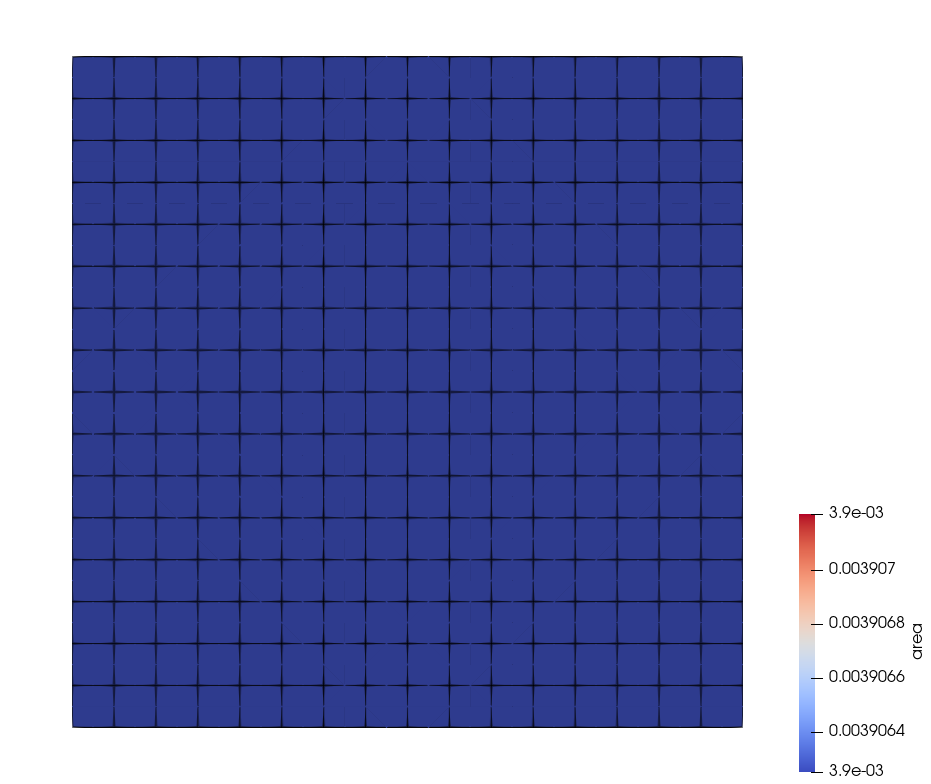
\includegraphics[width=5.5cm]{python_codes/fieldstone_76/results/mt1}
{\small 2})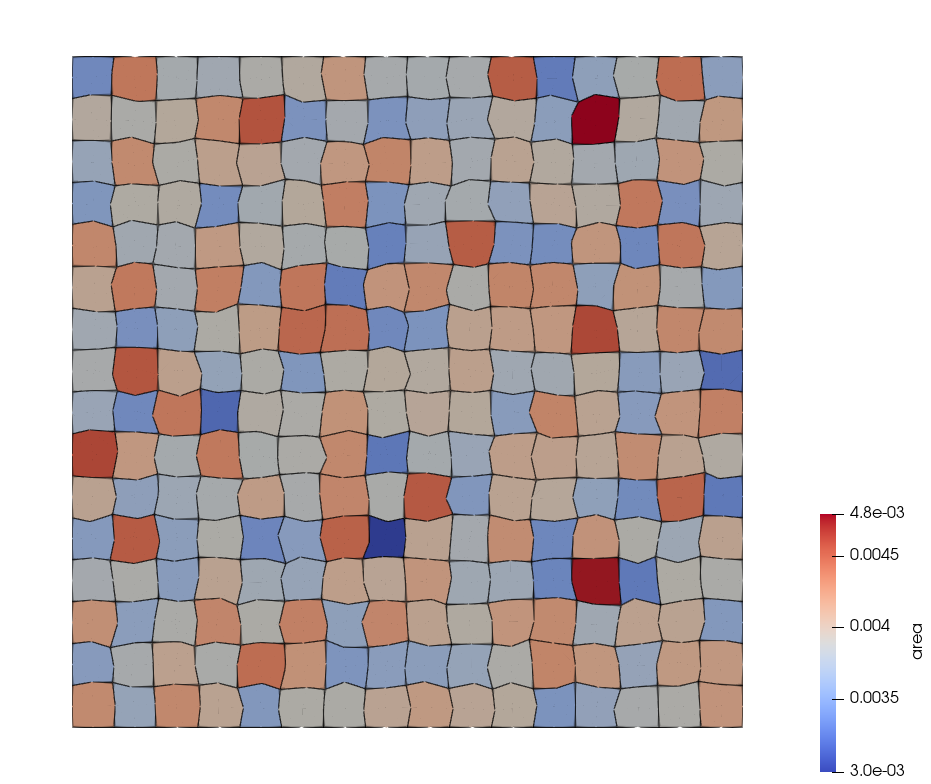
\includegraphics[width=5.5cm]{python_codes/fieldstone_76/results/mt2}
{\small 3})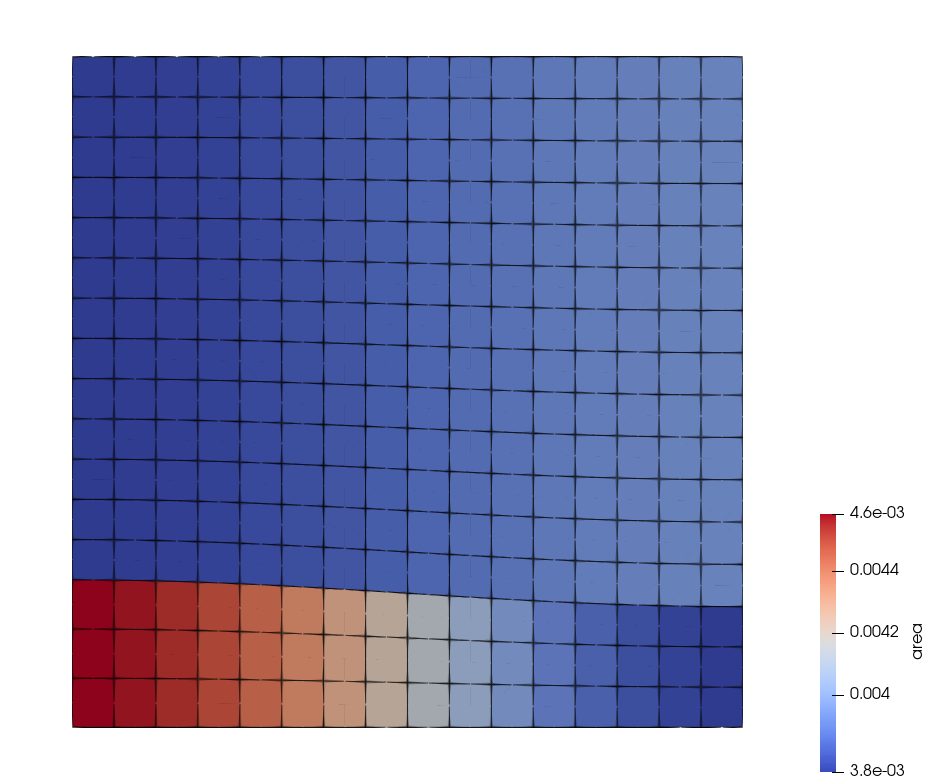
\includegraphics[width=5.5cm]{python_codes/fieldstone_76/results/mt3}\\
{\small 4})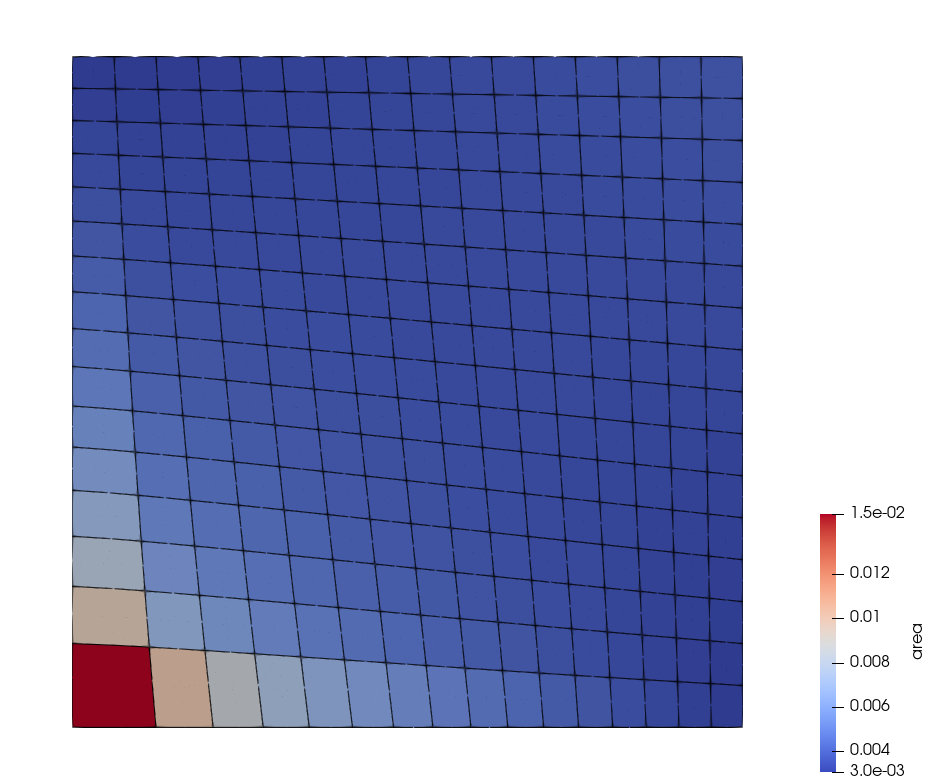
\includegraphics[width=5.5cm]{python_codes/fieldstone_76/results/mt4}
{\small 5})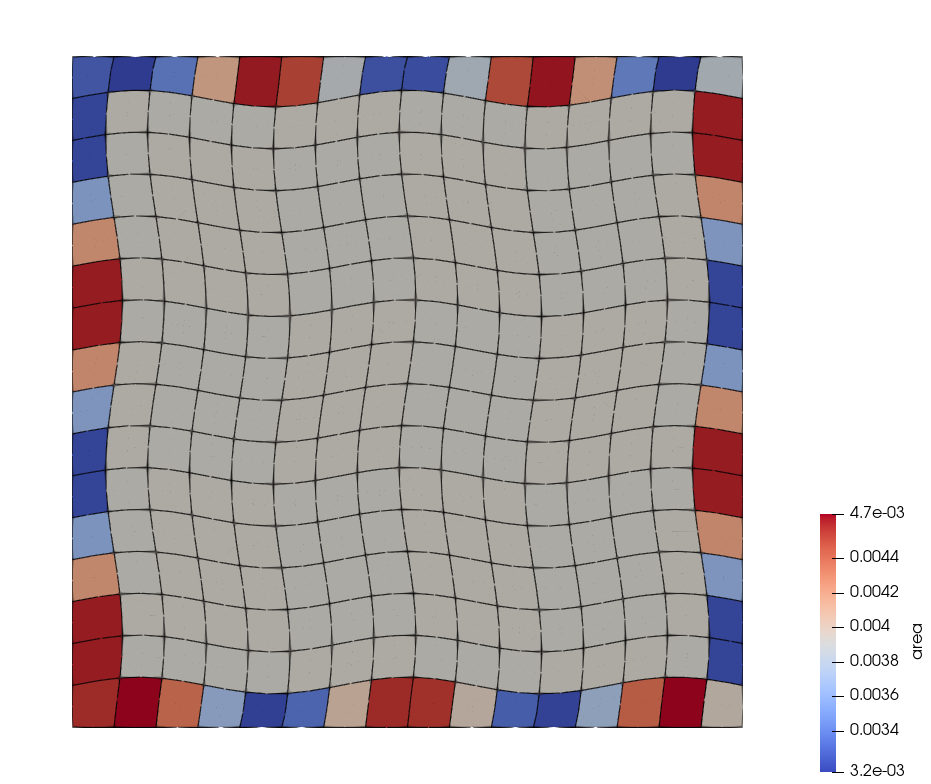
\includegraphics[width=5.5cm]{python_codes/fieldstone_76/results/mt5}
{\small 6})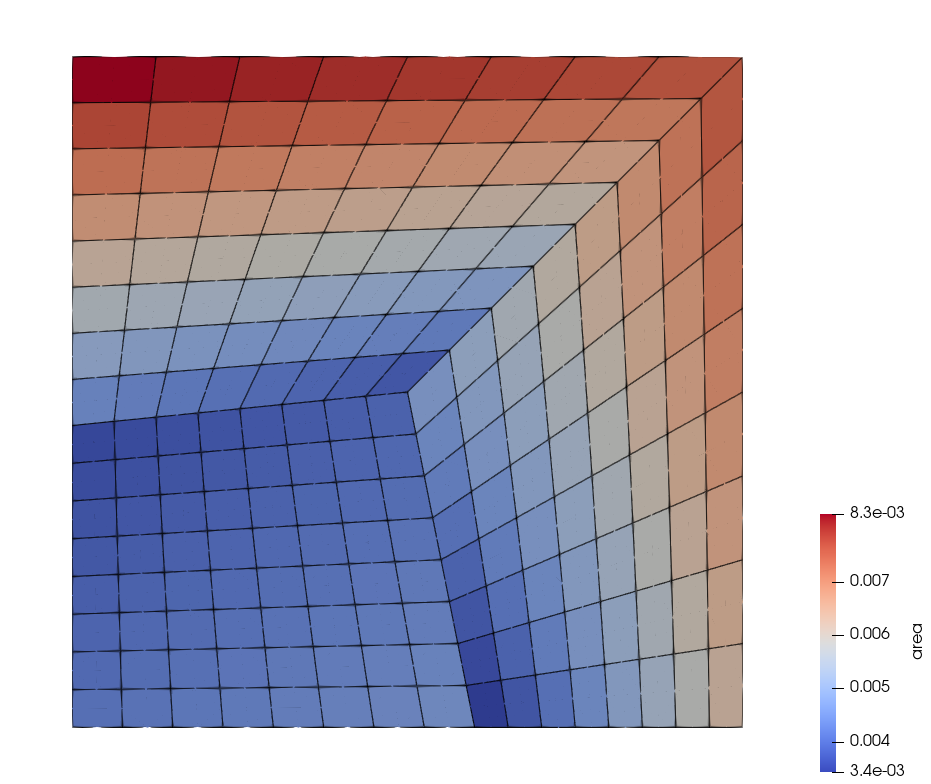
\includegraphics[width=5.5cm]{python_codes/fieldstone_76/results/mt6}\\
{\captionfont From left to right, top to bottom: mesh types 1, 2, 3, 4, 5 and 6, 
or 'square', 'randomized', 'wave', 'stretched', 'sin-sin' and 'glued' meshes.}
\end{center}

Looking at the meshes above we find that the cells of the 'wave' mesh 
can be obtained by affine transformation\footnote{\url{https://en.wikipedia.org/wiki/Affine_transformation}} 
of the reference cell (if straight edges are used -- see next paragraph) 
but not the cells of the 'randomized', 'stretched' and 'sin-sin' mesh. 
Quickly: an affine transformation 
is a geometric transformation that preserves lines and parallelism, but not necessarily 
Euclidean distances and angles. 
I remember coming across this terminology in the relevant literature (which I need to find again!)
and this may explain the results obtained for the manufactured solutions I ran the code on 
in what follows on both these types of meshes.

If the parameter \lstinline{straight_edges} is set to \lstinline{True}
the following algorithm makes sure that the velocity nodes 4,5,6,7 in the middle of the edges 
are really put back between nodes 0-1, 1-2, 2-3, and 3-0 respectively. 
\begin{lstlisting}
for iel in range(0,nel):
    xV[iconV[4,iel]]=0.5*(xV[iconV[0,iel]]+xV[iconV[1,iel]])
    yV[iconV[4,iel]]=0.5*(yV[iconV[0,iel]]+yV[iconV[1,iel]])
    xV[iconV[5,iel]]=0.5*(xV[iconV[1,iel]]+xV[iconV[2,iel]])
    yV[iconV[5,iel]]=0.5*(yV[iconV[1,iel]]+yV[iconV[2,iel]])
    xV[iconV[6,iel]]=0.5*(xV[iconV[2,iel]]+xV[iconV[3,iel]])
    yV[iconV[6,iel]]=0.5*(yV[iconV[2,iel]]+yV[iconV[3,iel]])
    xV[iconV[7,iel]]=0.5*(xV[iconV[3,iel]]+xV[iconV[0,iel]])
    yV[iconV[7,iel]]=0.5*(yV[iconV[3,iel]]+yV[iconV[0,iel]])
\end{lstlisting}
The placement of the middle node 8 is discussed in what follows.


The mapping is isoparametric (i.e. $Q_2$). The same mapping is used for changes 
of variables and for all integrals, Jacobians, etc ...
In the case of rectangular cells both the mapped and unmapped approaches 
yield the same pressure basis functions values at the quadrature points
so the measured errors are identical.
I suspected this is true for all cells obtained by affine transformation
from reference cell, to which my asking about this, W.B. added:
\begin{displayquote}
{\color{darkgray}
``Affine'' in essence means ``almost linear''. A linear transformation $f(x)$
satisfies $f(x+y) = f(x)+f(y)$ and  $f(\alpha x) = \alpha f(x)$
which in particular implies that $f(0)=0$. 
In finite-dimensional vector spaces, every linear transformation can be written as
$ f(x) = Ax $ with a matrix $A$. 

Affine transformations are of the form $f(x) = Ax + b$
which you need in the finite element context of affine transformations because
you don't just want to stretch or rotate cells, but you also want to translate
them from the reference coordinate system to wherever the cell is located in
real space.

If you have only rectangular cells (in fact, if they are parallelograms, of
which rectangles are a special case), then indeed the mapping is affine. The
shape functions in the mapped and unmapped case are different, but they span
the same space. (The shape functions are linear in both cases, but they are
scaled differently.) As a consequence, the solution is indeed the same. Like
you suggest in your question, this is going to be true for any affine
(=parallelogram) cell. It is because when you map linear basis functions with
an affine mapping, you end up with linear basis functions; the unmapped case
starts with linear shape functions in real space. 
}
\end{displayquote}

The same quadrature rule is used for $\K$ and $\G$ blocks (called $A$ and $B$ blocks 
respectively in the ASPECT literature).
I have explored the effect of the number of quadrature points on the solution, 
by testing for $2^2$, $3^2$ and $4^2$ quadrature points
as parameterized by the \lstinline{nqperdim} parameter.
I unsurprisingly found that a $2^2$ is not sufficient to exactly integrate the 
terms found in the $\K$ and $\G$ blocks, $3^2$ is standard, 
and $4^2$ is wasteful and did not yield any change in the results compared to $3^2$.

One critical aspect of the implementation is the location of the pressure nodes
in the real cell. The code takes the following approach:
\begin{enumerate}
\item For each cell compute the coordinates of the velocity nodes 0-7,
\item Apply modifications to the mesh (stretching, randomization, ...),
\item Set location of (middle) velocity node 8 (see next section),
\item Use $Q_2$ mapping to compute $x,y$ coordinates of pressure nodes.
\end{enumerate}


In both cases (mapped and unmapped) the pressure is discontinuous from cell to cell 
and this adds complexity in terms of exporting it to vtu format (and plotting with paraview). 
I then simply choose to export the value of the pressure in the middle of 
each cell\footnote{I should improve this in the future, but it is 
only a visualisation problem and does not influence results.
I know how to fix it, but this has low priority.}

%............................................................................
\subsubsection{About the position of the middle node}

We can think of multiple ways to come up with the `center' of the cell, 
i.e. the location of node 8.

\begin{verbatim}
3--6--2 
|     | 
7  8  5 
|     | 
0--4--1 
V nodes 
\end{verbatim}

In the code these different approaches are parameterized by means of the
\lstinline{center} variable:

\begin{itemize}
\item \lstinline{center=0}: The middle node coordinates are simply the 
average of the corner coordinates 
\begin{align}
x_8&=(x_0+x_1+x_2+x_3)/4 \nn\\
y_8&=(y_0+y_1+y_2+y_3)/4 \nn
\end{align}

\item \lstinline{center=1}: The middle coordinates are the average all the 
4 corners and 4 mid-edge nodes coordinates:

\begin{align}
x_8&=(x_0+x_1+x_2+x_3+x_4+x_5+x_6+x_7)/8 \nn\\
y_8&=(y_0+y_1+y_2+y_3+y_4+y_5+y_6+y_7)/8 \nn
\end{align}

\item \lstinline{center=2}: The middle coordinates are obtained via a 
weighed sum of the corner coordinates and the mid-edge nodes 
coordinates\footnote{I have no idea where this comes from but left it in nevertheless.}: 

\begin{align}
x_8&=(x_0+x_1+x_2+x_3+3x_4+3x_5+3x_6+3x_7)/16. \nn\\
y_8&=(y_0+y_1+y_2+y_3+3y_4+3y_5+3y_6+3y_7)/16. \nn
\end{align}

\item \lstinline{center=3}: This approach is a bit more complex than the previous ones.
We start by acknowledging that we know the coordinates of nodes 0-7 in the reference space $(r,s)$ 
and in the real space $(x,y)$ so one could then use a $Q_2^{(8)}$ mapping (i.e. 'serendipity' $Q_2$)
to place node 8.

In this case the basis functions for this mapping are defined in Section~\ref{MMM-sec:serendipity2D}:
\begin{eqnarray}
\bN_0(r,s)&=& \frac{1}{4}(1-r)(1-s)(-r-s-1) \nn\\
\bN_1(r,s)&=& \frac{1}{4}(1+r)(1-s)(r-s-1) \nn\\
\bN_2(r,s)&=& \frac{1}{4}(1+r)(1+s)(r+s-1) \nn\\
\bN_3(r,s)&=& \frac{1}{4}(1-r)(1+s)(-r+s-1) \nn\\
\bN_4(r,s)&=& \frac{1}{2}(1-r^2)(1-s)  \nn\\
\bN_5(r,s)&=& \frac{1}{2}(1+r)  (1-s^2)\nn\\
\bN_6(r,s)&=& \frac{1}{2}(1-r^2)(1+s)  \nn\\
\bN_7(r,s)&=& \frac{1}{2}(1-r)  (1-s^2) \nn
\end{eqnarray}

We would then compute the location of node 8 as follows (its $r,s$ coordinates are $0,0$): 
\begin{eqnarray}
x_8
&=& \sum_{i=0}^7 \bN_i (r_8,s_8) x_i \nn\\
&=& \sum_{i=1}^7 \bN_i (0,0) x_i \nn\\
&=& -\frac14 (x_0+x_1+x_2+x_3) + \frac12 (x_4+x_5+x_6+x_7) \nn\\
y_8 
&=& \sum_{i=0}^7 \bN_i (r_8,s_8) y_i \nn\\
&=& \sum_{i=0}^7 \bN_i (0,0) y_i \nn\\
&=& -\frac14 (y_0+y_1+y_2+y_3) + \frac12 (y_4+y_5+y_6+y_7) \nn
\end{eqnarray}

\end{itemize}

In the case of parallelogram cells these four approaches lead to the same 
middle location. This is no more the case for elements with curved edges
for example and therefore warrants a thorough study.

%--------------------------------------------------------------------------------------
\subsection*{The manufactured solutions}

Note that for all four manufactured solutions used in the present code 
a) the pressure obeys $\int_{\Omega} p \; dV = 0$;
b) the analytical velocity is prescribed on the boundary of the domain; 
c) the viscosity is 1 (except SolKz); d) the domain is the unit square. 

\begin{itemize}
\item {\tt bench=3}: 
This is the Donea \& Huerta benchmark that is fully described in Section~\ref{MMM-mms1}.
The velocity and pressure are given by
\begin{eqnarray}
u(x,y) &=& x^2(1-x)^2 2y (y-1)(2y-1) \\ 
v(x,y) &=& -y^2 (1 - y)^2 2x (x-1)(2x-1) \\ 
p(x,y) &=& x(1 -x)- 1/6 
\end{eqnarray}

\item {\tt bench=1}:  
The analytical solution originates in Lamichhane (2017) \cite{lami17}.
The velocity and pressure are given by
\begin{eqnarray}
u(x,y)&=&-2x^2y(2y-1)(x-1)^2(y-1) \\
v(x,y)&=& 2xy^2(2x-1)(x-1)(y-1)^2 \\
p(x,y)&=& x(1-x)(1-2y)
\end{eqnarray}
The corresponding body force terms are derived in Section~\ref{MMM-ss:mms11}. 

\item {\tt bench=9}: 
This is the second manufactured solution 
mentioned in Lamichhane \cite{lami17}. 
The velocity and pressure are given by
\begin{eqnarray}
u(x,y) &=& x+x^2 - 2xy+x^3 - 3xy^2 + x^2y \\
v(x,y) &=& -y-2xy+y^2 -3x^2y + y^3 - xy^2 \\
p(x,y) &=& xy+x+y+x^3y^2 - 4/3
\end{eqnarray}
The corresponding body force terms are derived in Section~\ref{MMM-ss:mms2}. 

\item {\tt bench=4}. This is the SolKz benchmark described in Section~\ref{MMM-ss:solkz}.
The main difference with respect to the previous three ones is the fact that the viscosity
varies by 6 orders of magnitude (albeit is a smooth manner).


\end{itemize}

The numbering {\tt bench=3,1,9,4} is completely arbitrary and inherited from another \stone.

In what follows velocity and pressure error convergence is measured as a function of
mesh side. Since for some meshes there is not a single obvious mesh size, 
I then use the square root of the maximum value of the elemental area array:
\[
h \simeq \sqrt{\max_e A_e }
\]


\newpage
%--------------------------------------------------------------------------------------
\subsection*{Manufactured solution of Donea \& Huerta ({\tt bench=3}) - straight edges}

\begin{center}
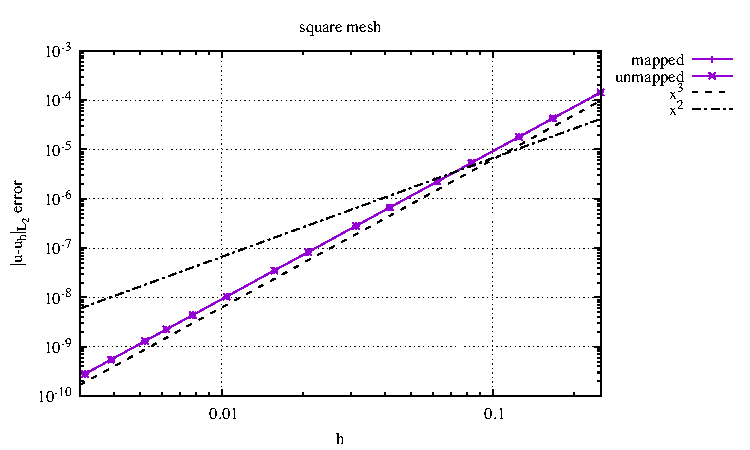
\includegraphics[width=6.5cm]{python_codes/fieldstone_76/results/bench3/straight/errors_V_mt1.pdf}
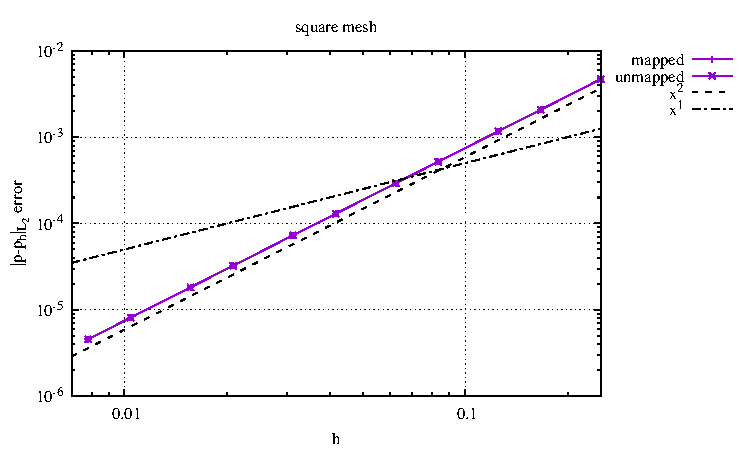
\includegraphics[width=6.5cm]{python_codes/fieldstone_76/results/bench3/straight/errors_P_mt1.pdf}\\
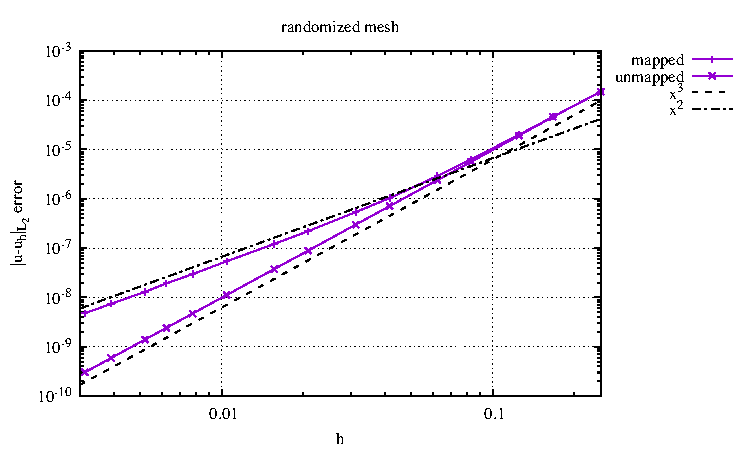
\includegraphics[width=6.5cm]{python_codes/fieldstone_76/results/bench3/straight/errors_V_mt2.pdf}
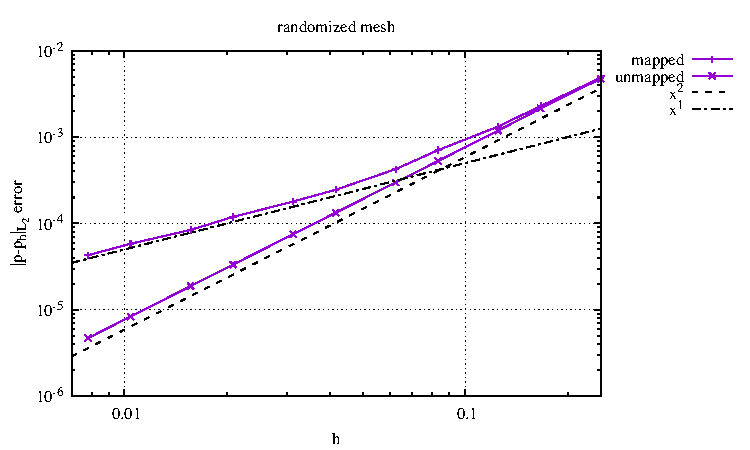
\includegraphics[width=6.5cm]{python_codes/fieldstone_76/results/bench3/straight/errors_P_mt2.pdf}\\
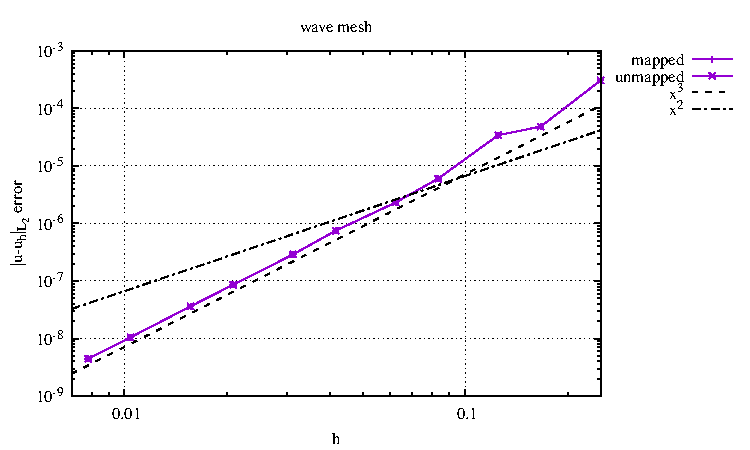
\includegraphics[width=6.5cm]{python_codes/fieldstone_76/results/bench3/straight/errors_V_mt3.pdf}
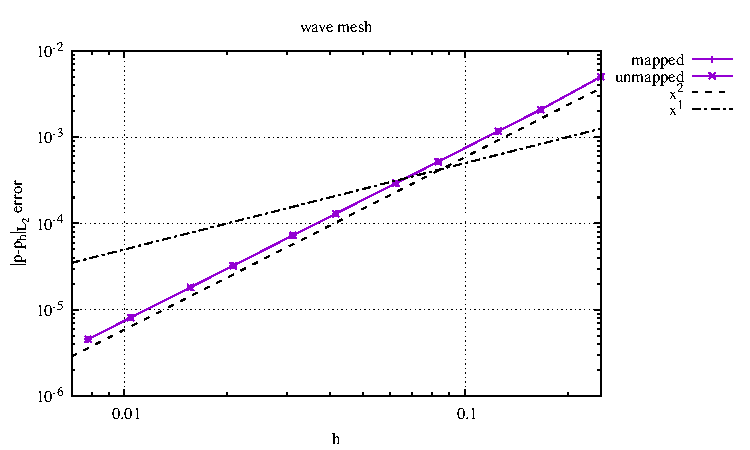
\includegraphics[width=6.5cm]{python_codes/fieldstone_76/results/bench3/straight/errors_P_mt3.pdf}\\
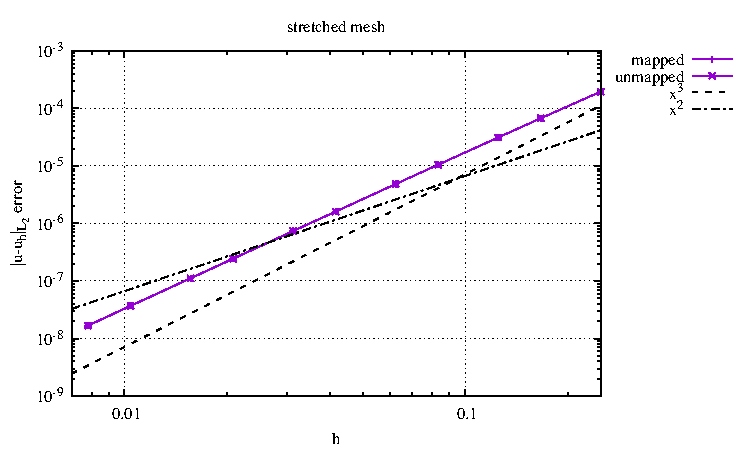
\includegraphics[width=6.5cm]{python_codes/fieldstone_76/results/bench3/straight/errors_V_mt4.pdf}
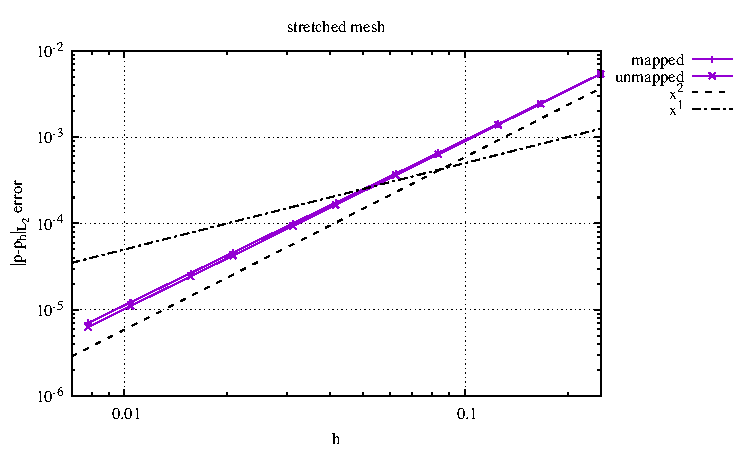
\includegraphics[width=6.5cm]{python_codes/fieldstone_76/results/bench3/straight/errors_P_mt4.pdf}\\
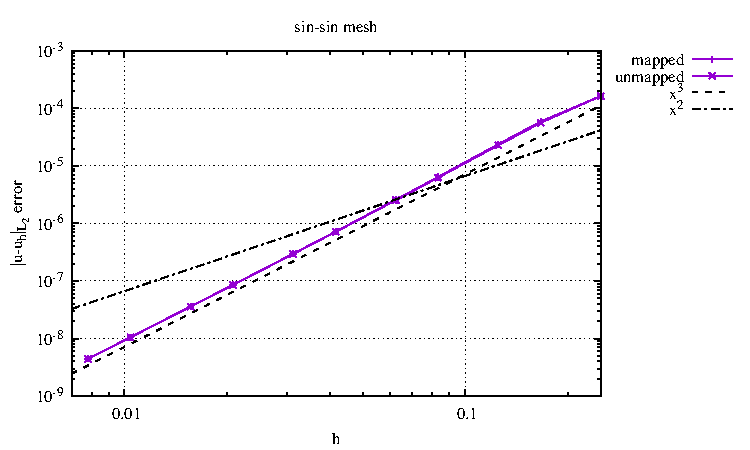
\includegraphics[width=6.5cm]{python_codes/fieldstone_76/results/bench3/straight/errors_V_mt5.pdf}
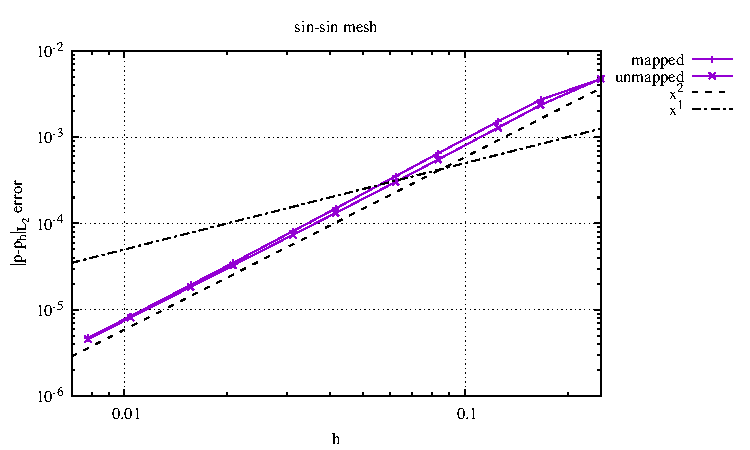
\includegraphics[width=6.5cm]{python_codes/fieldstone_76/results/bench3/straight/errors_P_mt5.pdf}\\
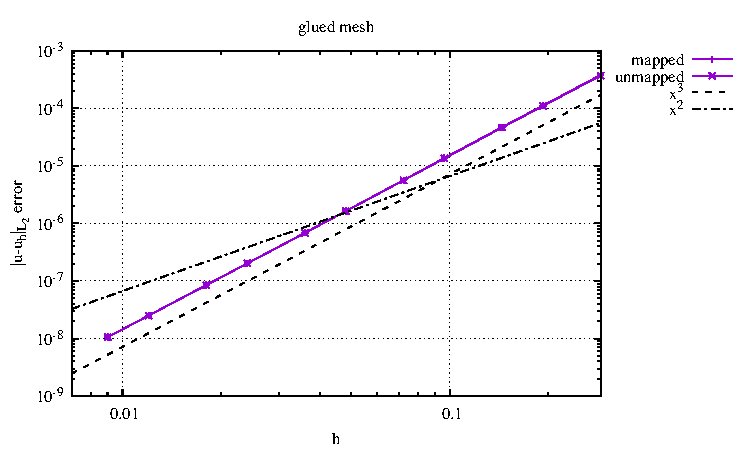
\includegraphics[width=6.5cm]{python_codes/fieldstone_76/results/bench3/straight/errors_V_mt6.pdf}
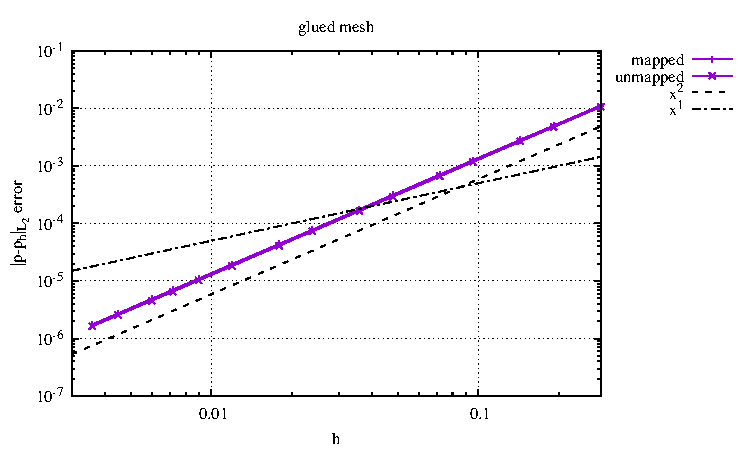
\includegraphics[width=6.5cm]{python_codes/fieldstone_76/results/bench3/straight/errors_P_mt6.pdf}\\
{\captionfont From top to bottom: square mesh, Randomized ($\xi=0.1$) mesh,
wave mesh, stretched mesh, sin-sin mesh and glued mesh.}
\end{center}

\newpage
%------------------------------------------------------------------------------------
\subsection*{Manufactured solution of Donea \& Huerta ({\tt bench=3}) - curved edges}

\begin{center}
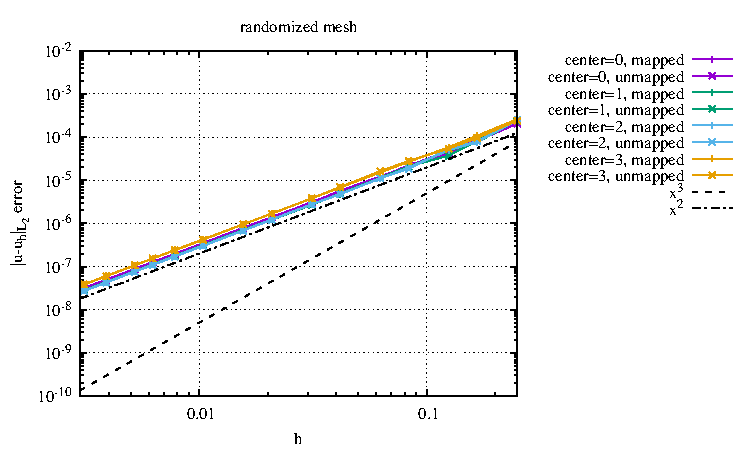
\includegraphics[width=8cm]{python_codes/fieldstone_76/results/bench3/curved/errors_V_mt2.pdf}
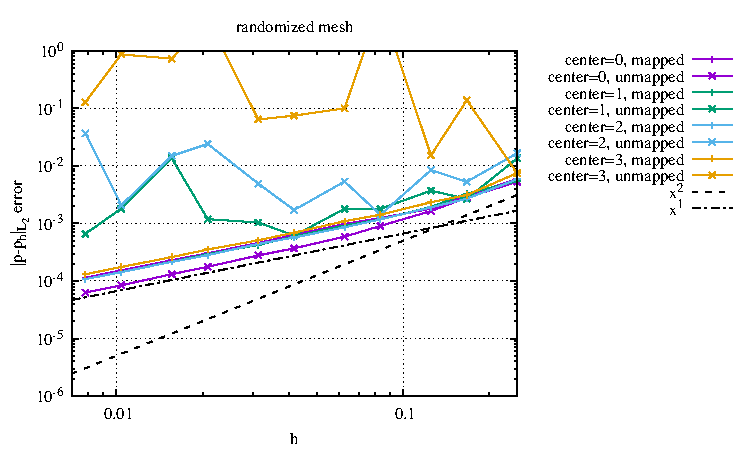
\includegraphics[width=8cm]{python_codes/fieldstone_76/results/bench3/curved/errors_P_mt2.pdf}\\
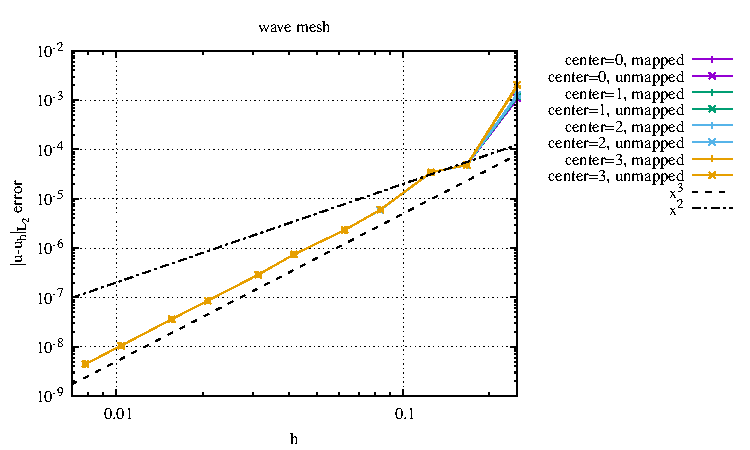
\includegraphics[width=8cm]{python_codes/fieldstone_76/results/bench3/curved/errors_V_mt3.pdf}
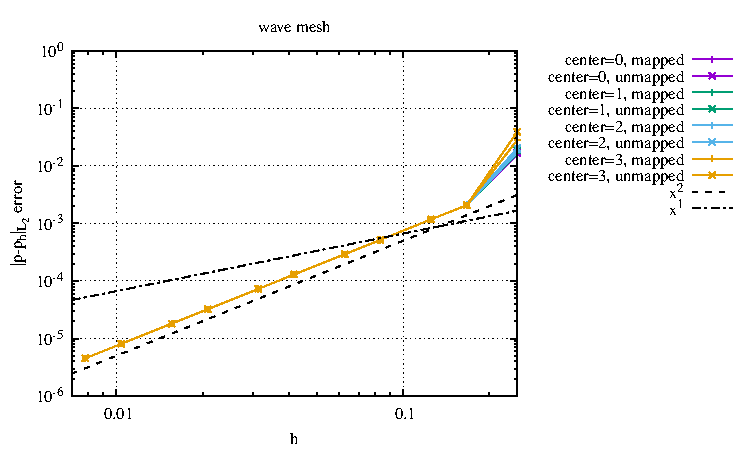
\includegraphics[width=8cm]{python_codes/fieldstone_76/results/bench3/curved/errors_P_mt3.pdf}\\
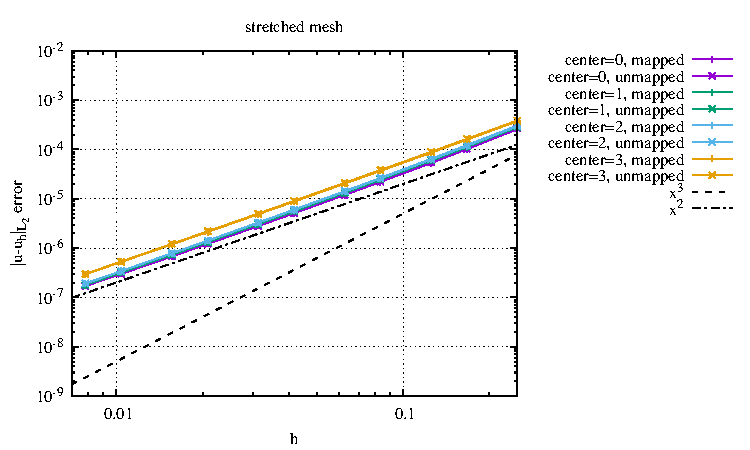
\includegraphics[width=8cm]{python_codes/fieldstone_76/results/bench3/curved/errors_V_mt4.pdf}
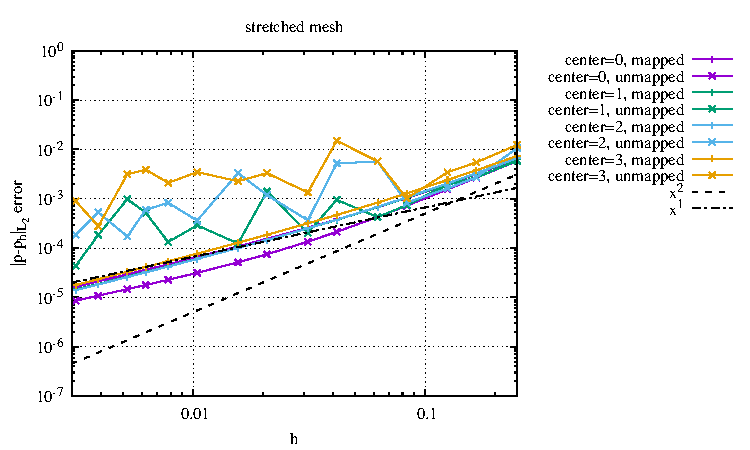
\includegraphics[width=8cm]{python_codes/fieldstone_76/results/bench3/curved/errors_P_mt4.pdf}\\
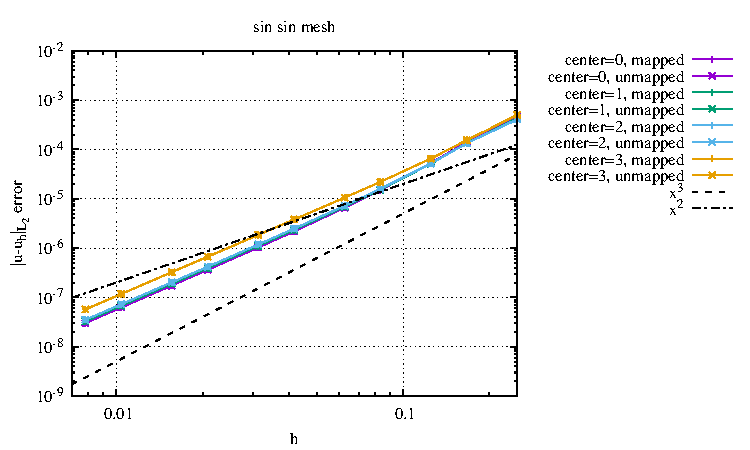
\includegraphics[width=8cm]{python_codes/fieldstone_76/results/bench3/curved/errors_V_mt5.pdf}
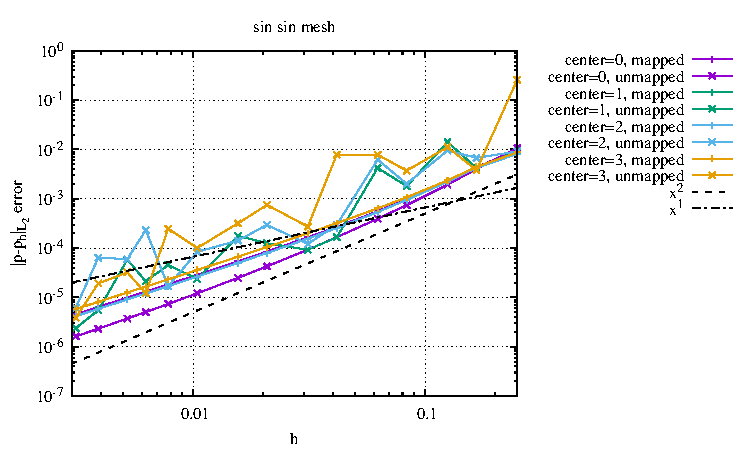
\includegraphics[width=8cm]{python_codes/fieldstone_76/results/bench3/curved/errors_P_mt5.pdf}\\
{\captionfont From top to bottom: 'randomized' ($\xi=0.1$) mesh,
'wave' mesh, 'stretched' mesh and 'sin-sin' mesh.}
\end{center}

\newpage
%-----------------------------------------------------------------------
\subsection*{Manufactured solution \#1 ({\tt bench=1}) - straight edges}

\begin{center}
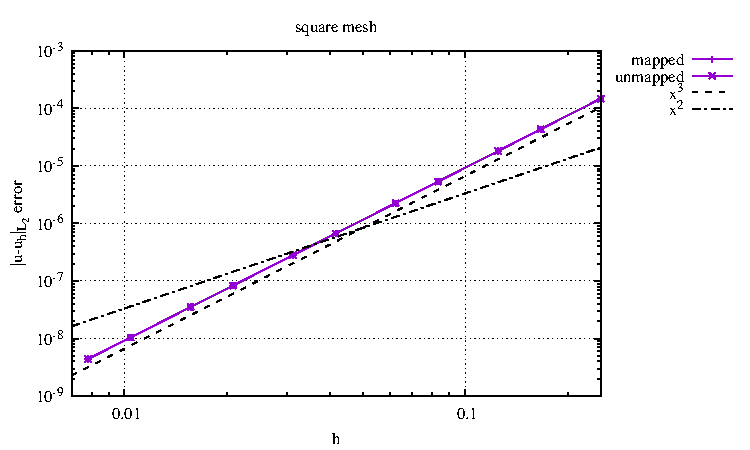
\includegraphics[width=6.5cm]{python_codes/fieldstone_76/results/bench1/straight/errors_V_mt1.pdf}
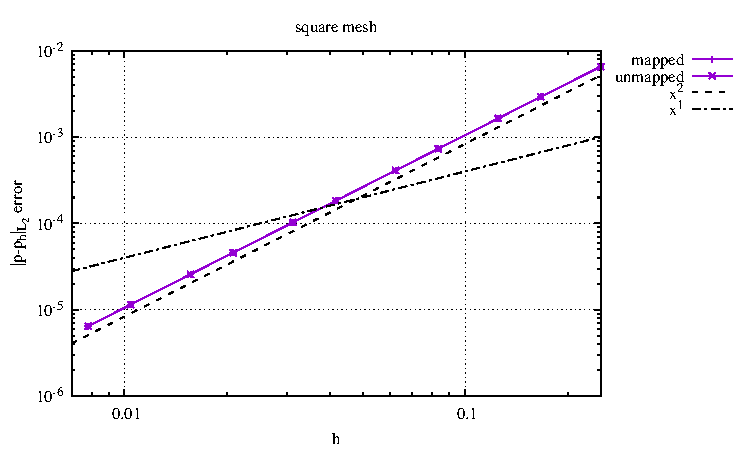
\includegraphics[width=6.5cm]{python_codes/fieldstone_76/results/bench1/straight/errors_P_mt1.pdf}\\
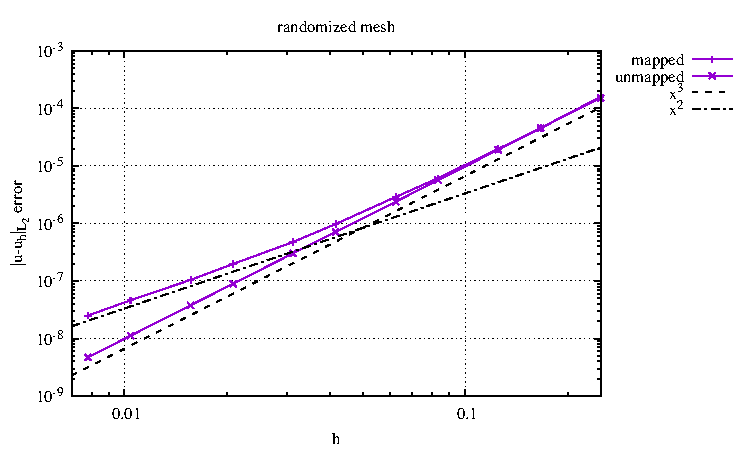
\includegraphics[width=6.5cm]{python_codes/fieldstone_76/results/bench1/straight/errors_V_mt2.pdf}
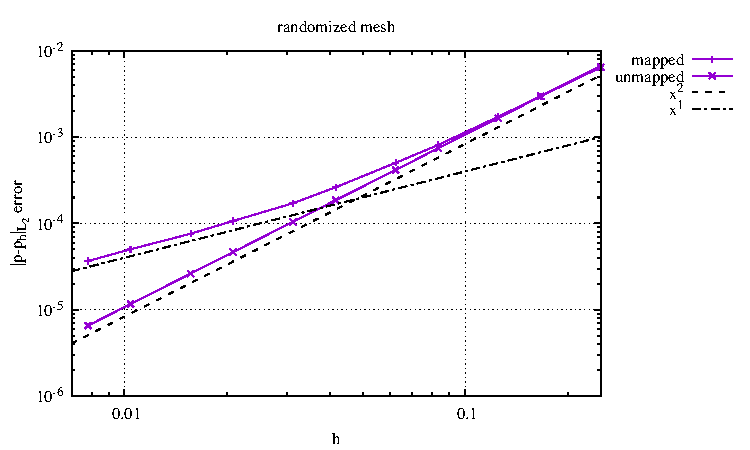
\includegraphics[width=6.5cm]{python_codes/fieldstone_76/results/bench1/straight/errors_P_mt2.pdf}\\
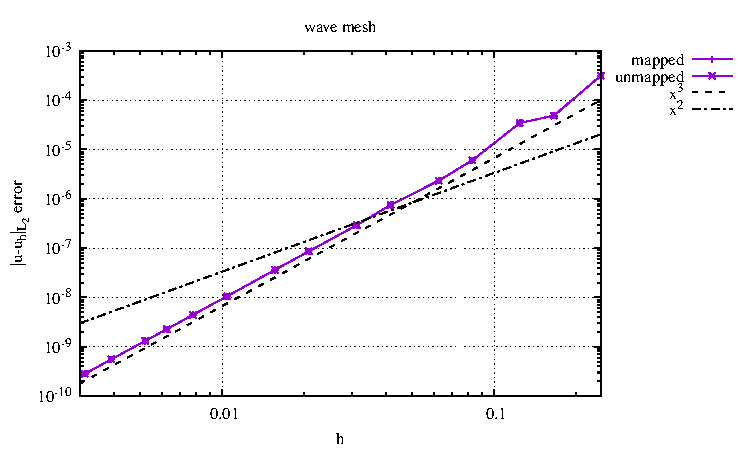
\includegraphics[width=6.5cm]{python_codes/fieldstone_76/results/bench1/straight/errors_V_mt3.pdf}
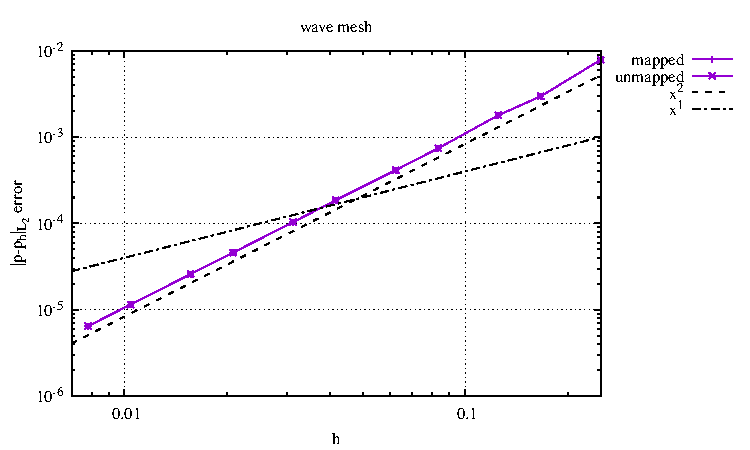
\includegraphics[width=6.5cm]{python_codes/fieldstone_76/results/bench1/straight/errors_P_mt3.pdf}\\
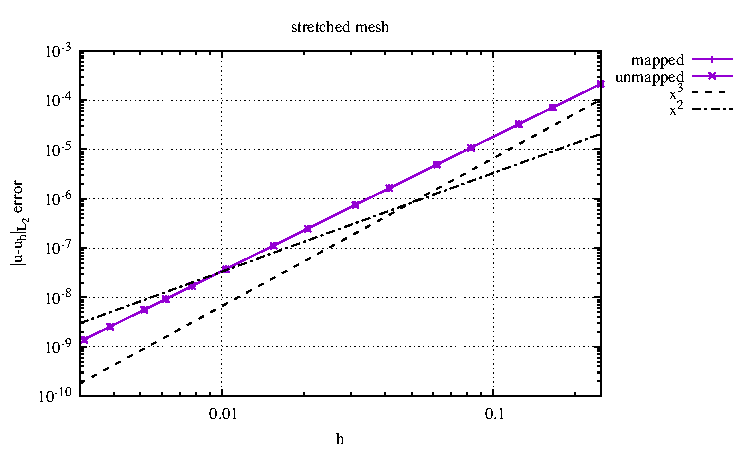
\includegraphics[width=6.5cm]{python_codes/fieldstone_76/results/bench1/straight/errors_V_mt4.pdf}
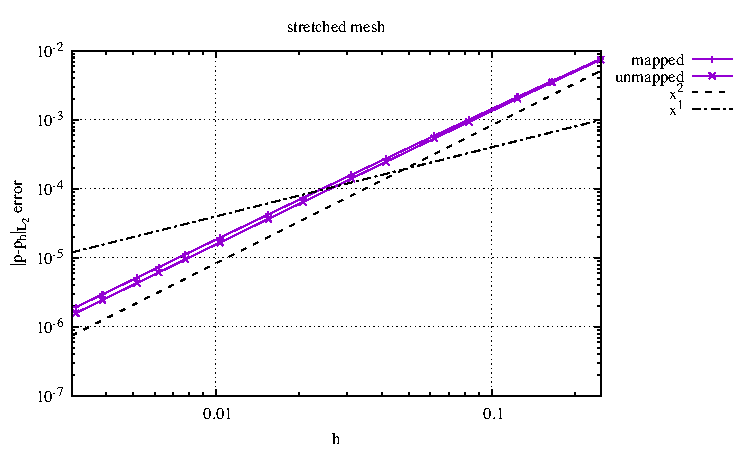
\includegraphics[width=6.5cm]{python_codes/fieldstone_76/results/bench1/straight/errors_P_mt4.pdf}\\
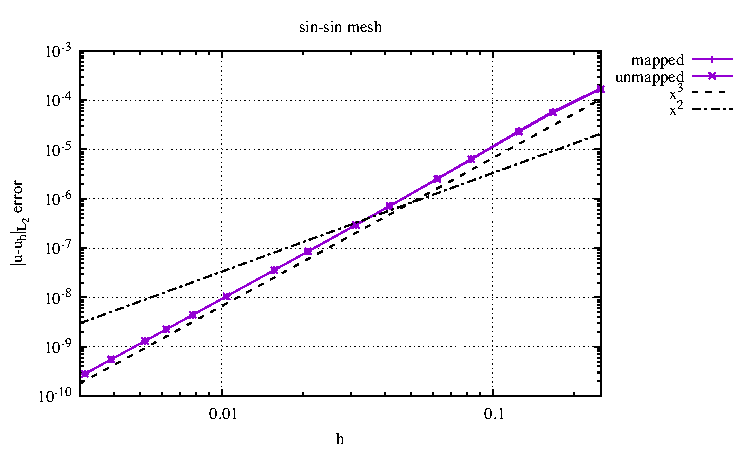
\includegraphics[width=6.5cm]{python_codes/fieldstone_76/results/bench1/straight/errors_V_mt5.pdf}
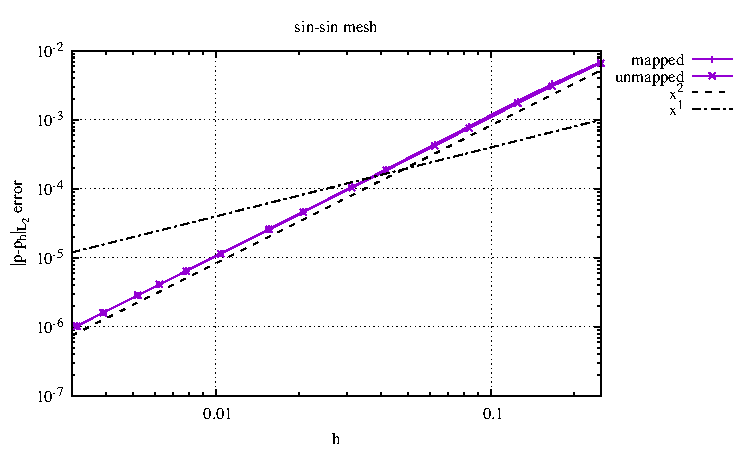
\includegraphics[width=6.5cm]{python_codes/fieldstone_76/results/bench1/straight/errors_P_mt5.pdf}\\
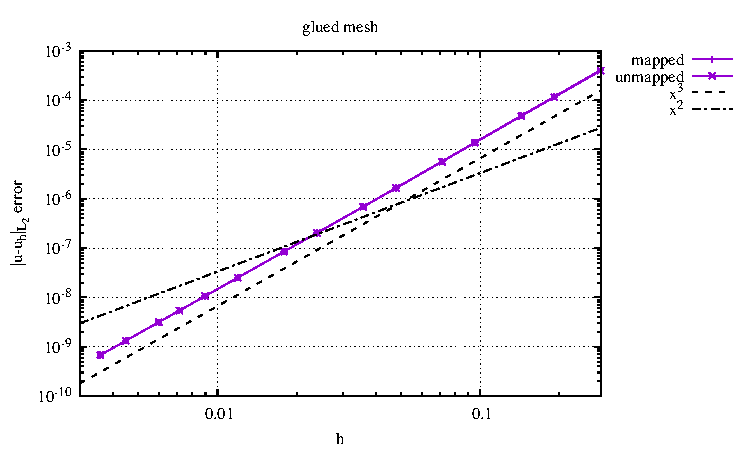
\includegraphics[width=6.5cm]{python_codes/fieldstone_76/results/bench1/straight/errors_V_mt6.pdf}
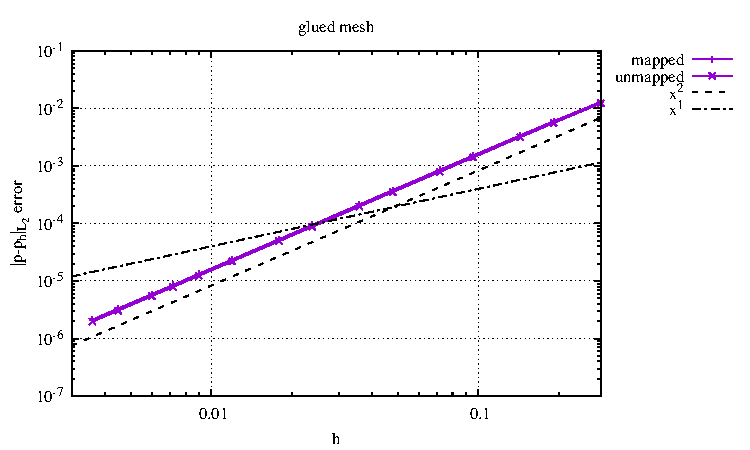
\includegraphics[width=6.5cm]{python_codes/fieldstone_76/results/bench1/straight/errors_P_mt6.pdf}\\
{\captionfont From top to bottom: 'square mesh', 'randomized' ($\xi=0.1$) mesh,
'wave' mesh, 'stretched' mesh, 'sin-sin' mesh and 'glued' mesh.}
\end{center}

\newpage
%.......................................................................
\subsection*{Manufactured solution \#1 ({\tt bench=1}) - curved edges}

\begin{center}
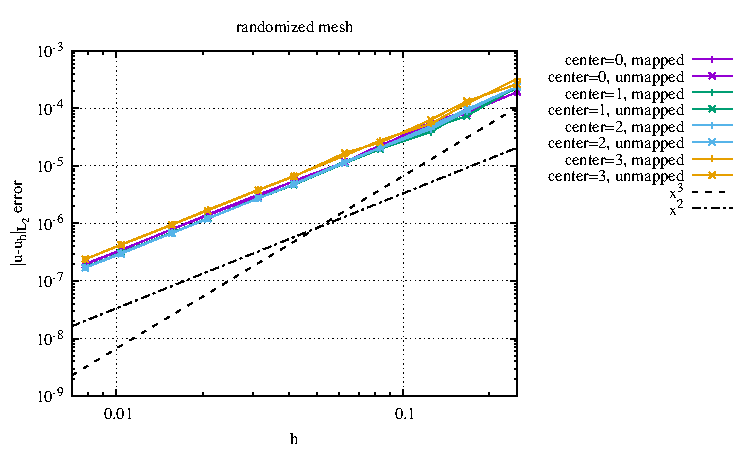
\includegraphics[width=8cm]{python_codes/fieldstone_76/results/bench1/curved/errors_V_mt2.pdf}
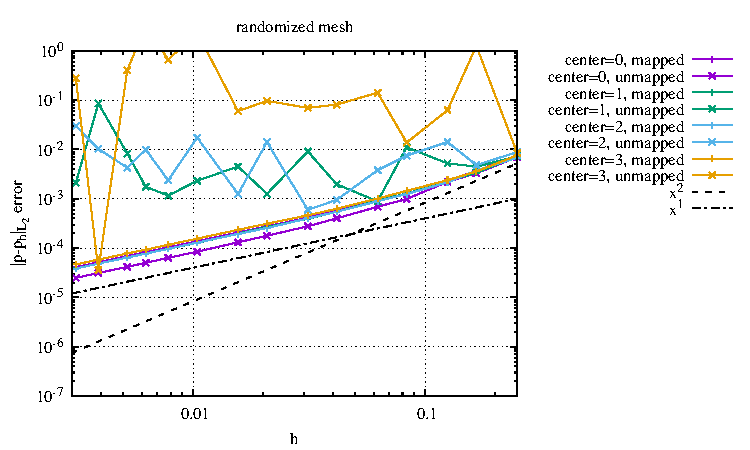
\includegraphics[width=8cm]{python_codes/fieldstone_76/results/bench1/curved/errors_P_mt2.pdf}\\
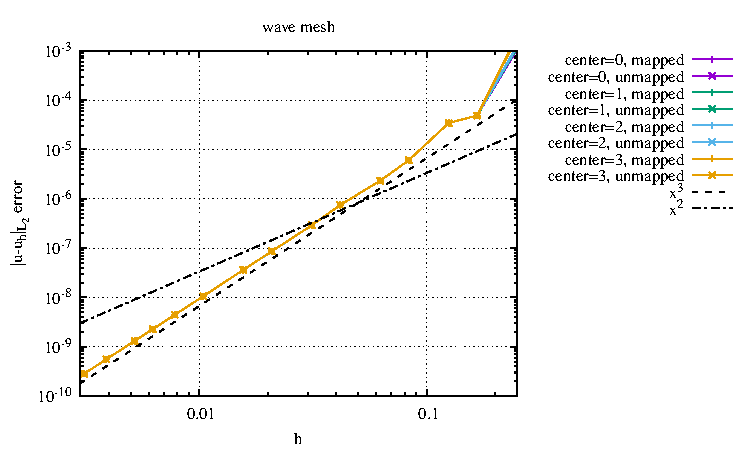
\includegraphics[width=8cm]{python_codes/fieldstone_76/results/bench1/curved/errors_V_mt3.pdf}
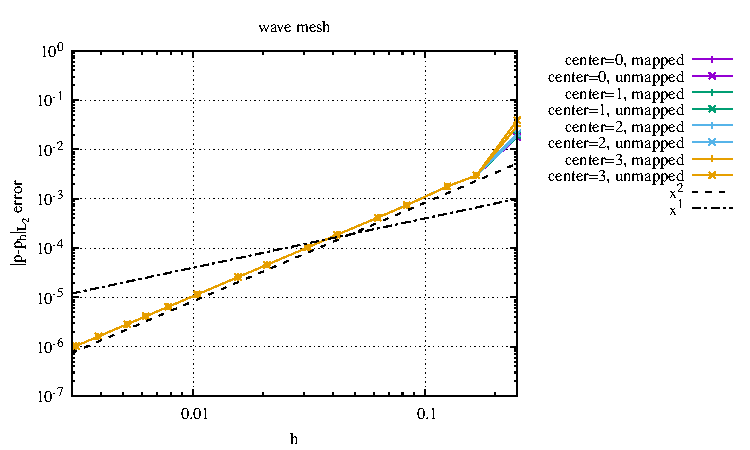
\includegraphics[width=8cm]{python_codes/fieldstone_76/results/bench1/curved/errors_P_mt3.pdf}\\
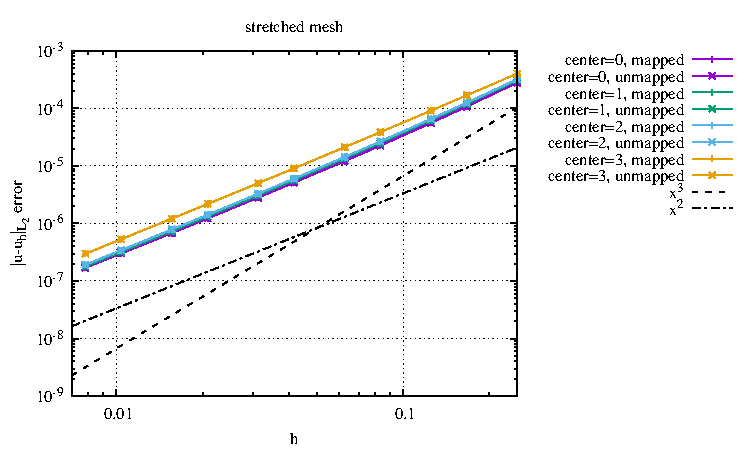
\includegraphics[width=8cm]{python_codes/fieldstone_76/results/bench1/curved/errors_V_mt4.pdf}
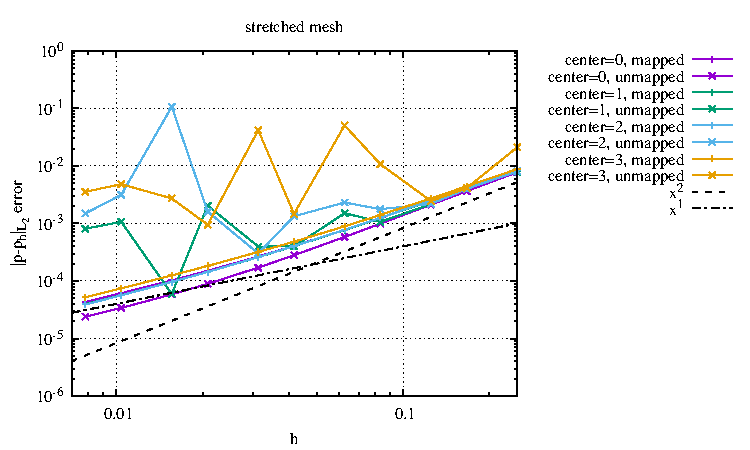
\includegraphics[width=8cm]{python_codes/fieldstone_76/results/bench1/curved/errors_P_mt4.pdf}\\
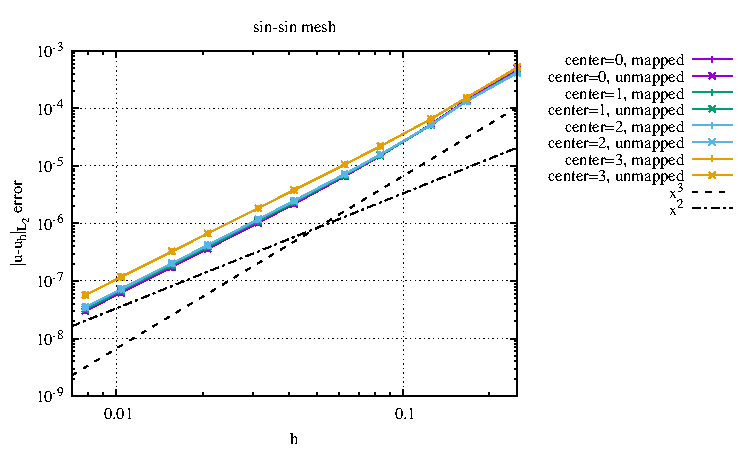
\includegraphics[width=8cm]{python_codes/fieldstone_76/results/bench1/curved/errors_V_mt5.pdf}
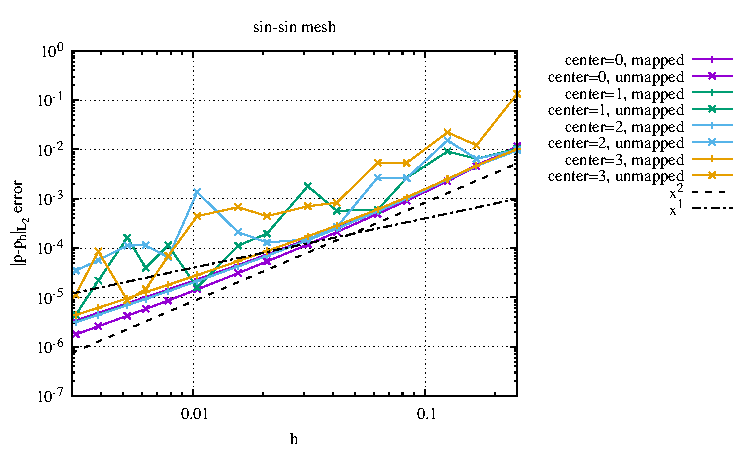
\includegraphics[width=8cm]{python_codes/fieldstone_76/results/bench1/curved/errors_P_mt5.pdf}\\
{\captionfont From top to bottom: 'randomized' ($\xi=0.1$) mesh,
'wave' mesh, 'stretched' mesh and 'sin-sin' mesh.}
\end{center}


\newpage
%.......................................................................
\subsection*{Manufactured solution \#2 ({\tt bench=9}) - straight edges}

\begin{center}
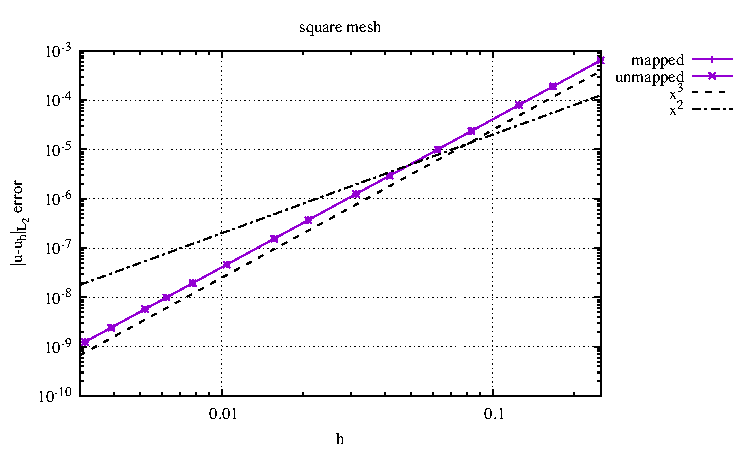
\includegraphics[width=6.5cm]{python_codes/fieldstone_76/results/bench9/straight/errors_V_mt1.pdf}
\includegraphics[width=6.5cm]{python_codes/fieldstone_76/results/bench9/straight/errors_P_mt1.pdf}\\
\includegraphics[width=6.5cm]{python_codes/fieldstone_76/results/bench9/straight/errors_V_mt2.pdf}
\includegraphics[width=6.5cm]{python_codes/fieldstone_76/results/bench9/straight/errors_P_mt2.pdf}\\
\includegraphics[width=6.5cm]{python_codes/fieldstone_76/results/bench9/straight/errors_V_mt3.pdf}
\includegraphics[width=6.5cm]{python_codes/fieldstone_76/results/bench9/straight/errors_P_mt3.pdf}\\
\includegraphics[width=6.5cm]{python_codes/fieldstone_76/results/bench9/straight/errors_V_mt4.pdf}
\includegraphics[width=6.5cm]{python_codes/fieldstone_76/results/bench9/straight/errors_P_mt4.pdf}\\
\includegraphics[width=6.5cm]{python_codes/fieldstone_76/results/bench9/straight/errors_V_mt5.pdf}
\includegraphics[width=6.5cm]{python_codes/fieldstone_76/results/bench9/straight/errors_P_mt5.pdf}\\
\includegraphics[width=6.5cm]{python_codes/fieldstone_76/results/bench9/straight/errors_V_mt6.pdf}
\includegraphics[width=6.5cm]{python_codes/fieldstone_76/results/bench9/straight/errors_P_mt6.pdf}\\
{\captionfont From top to bottom: 'square' mesh, 'randomized' ($\xi=0.1$) mesh,
'wave' mesh, 'stretched' mesh, 'sin-sin' mesh and 'glued' mesh.}
\end{center}

\newpage
%.......................................................................
\subsection*{Manufactured solution \#2 ({\tt bench=9}) - curved edges}

\begin{center}
\includegraphics[width=8cm]{python_codes/fieldstone_76/results/bench9/curved/errors_V_mt2.pdf}
\includegraphics[width=8cm]{python_codes/fieldstone_76/results/bench9/curved/errors_P_mt2.pdf}\\
\includegraphics[width=8cm]{python_codes/fieldstone_76/results/bench9/curved/errors_V_mt3.pdf}
\includegraphics[width=8cm]{python_codes/fieldstone_76/results/bench9/curved/errors_P_mt3.pdf}\\
\includegraphics[width=8cm]{python_codes/fieldstone_76/results/bench9/curved/errors_V_mt4.pdf}
\includegraphics[width=8cm]{python_codes/fieldstone_76/results/bench9/curved/errors_P_mt4.pdf}\\
\includegraphics[width=8cm]{python_codes/fieldstone_76/results/bench9/curved/errors_V_mt5.pdf}
\includegraphics[width=8cm]{python_codes/fieldstone_76/results/bench9/curved/errors_P_mt5.pdf}\\
{\captionfont From top to bottom: 'randomized' ($\xi=0.1$) mesh,
'wave' mesh, 'stretched' mesh and 'sin-sin' mesh.}
\end{center}


\newpage
%.......................................................................
\subsection*{Manufactured solution SolKz ({\tt bench=4}) - straight edges}

\begin{center}
\includegraphics[width=6.5cm]{python_codes/fieldstone_76/results/bench4/straight/errors_V_mt1.pdf}
\includegraphics[width=6.5cm]{python_codes/fieldstone_76/results/bench4/straight/errors_P_mt1.pdf}\\
\includegraphics[width=6.5cm]{python_codes/fieldstone_76/results/bench4/straight/errors_V_mt2.pdf}
\includegraphics[width=6.5cm]{python_codes/fieldstone_76/results/bench4/straight/errors_P_mt2.pdf}\\
\includegraphics[width=6.5cm]{python_codes/fieldstone_76/results/bench4/straight/errors_V_mt3.pdf}
\includegraphics[width=6.5cm]{python_codes/fieldstone_76/results/bench4/straight/errors_P_mt3.pdf}\\
\includegraphics[width=6.5cm]{python_codes/fieldstone_76/results/bench4/straight/errors_V_mt4.pdf}
\includegraphics[width=6.5cm]{python_codes/fieldstone_76/results/bench4/straight/errors_P_mt4.pdf}\\
\includegraphics[width=6.5cm]{python_codes/fieldstone_76/results/bench4/straight/errors_V_mt5.pdf}
\includegraphics[width=6.5cm]{python_codes/fieldstone_76/results/bench4/straight/errors_P_mt5.pdf}\\
\includegraphics[width=6.5cm]{python_codes/fieldstone_76/results/bench4/straight/errors_V_mt6.pdf}
\includegraphics[width=6.5cm]{python_codes/fieldstone_76/results/bench4/straight/errors_P_mt6.pdf}\\
{\captionfont From top to bottom: 'square' mesh, 'randomized' ($\xi=0.1$) mesh,
'wave' mesh, 'stretched' mesh, 'sin-sin' mesh and 'glued' mesh.}
\end{center}

\newpage
%.......................................................................
\subsection*{Manufactured solution SolKz ({\tt bench=4}) - curved edges}

\begin{center}
\includegraphics[width=8cm]{python_codes/fieldstone_76/results/bench4/curved/errors_V_mt2.pdf}
\includegraphics[width=8cm]{python_codes/fieldstone_76/results/bench4/curved/errors_P_mt2.pdf}\\
\includegraphics[width=8cm]{python_codes/fieldstone_76/results/bench4/curved/errors_V_mt3.pdf}
\includegraphics[width=8cm]{python_codes/fieldstone_76/results/bench4/curved/errors_P_mt3.pdf}\\
\includegraphics[width=8cm]{python_codes/fieldstone_76/results/bench4/curved/errors_V_mt4.pdf}
\includegraphics[width=8cm]{python_codes/fieldstone_76/results/bench4/curved/errors_P_mt4.pdf}\\
\includegraphics[width=8cm]{python_codes/fieldstone_76/results/bench4/curved/errors_V_mt5.pdf}
\includegraphics[width=8cm]{python_codes/fieldstone_76/results/bench4/curved/errors_P_mt5.pdf} \\
{\captionfont From top to bottom: 'randomized' ($\xi=0.1$) mesh,
'wave' mesh, 'stretched' mesh and 'sin-sin' mesh.}
\end{center}


%%%%%%%%%%%%%%%%%%%%%%%%%%%%%%%%%%%%%%%%%%%%%%%%%%%%%%%%%%%%%%%%%%%%%%%%%%%%%%%%%%%%%%%%%%%%%
\newpage
\subsection*{A recap of all convergence rates so far}


As mentioned for example in \textcite{thba25} (2025), 
one expects a 3rd-order convergence (in the $L_2$ norm) for the velocity
error and a 2nd-order convergence for the pressure error.
In the tables below error rates that are not the expect 3/2 are highlighted in bold.

Since all four \lstinline{center} approaches are identical for straight edges
cells I will then only report values for \lstinline{center=0}. 



\begin{center}
\includegraphics[width=2.7cm]{python_codes/fieldstone_76/results/mt1}
\includegraphics[width=2.7cm]{python_codes/fieldstone_76/results/mt2}
\includegraphics[width=2.7cm]{python_codes/fieldstone_76/results/mt3}
\includegraphics[width=2.7cm]{python_codes/fieldstone_76/results/mt4}
\includegraphics[width=2.7cm]{python_codes/fieldstone_76/results/mt5}
\includegraphics[width=2.7cm]{python_codes/fieldstone_76/results/mt6}\\
{\captionfont 'square' ,'random', 'wave', 'stretched', 'sin-sin', 'glued'.}
\end{center}

\begin{itemize}

%...................................
\item {\tt bench=3}

\begin{tabular}{c|cccccc}
\hline
straight& mt=1     &  mt=2        &  mt=3  &  mt=4       & mt=5  & mt=6\\
edges& 'square' & 'randomized' & 'wave' & 'stretched' & 'sin-sin' & 'glued'\\
\hline
mapped   & 3/2 & {\bf 2/1} &3/2 & {\bf 2.74/1.88} &3/2 \\
unmapped & 3/2 &3/2 &3/2 & {\bf 2.74/1.92} &3/2 \\
\hline
\end{tabular}

\begin{tabular}{c|cccc}
\hline
curved &  mt=2        &  mt=3  &  mt=4       & mt=5 \\
edges & 'randomized' & 'wave' & 'stretched' & 'sin-sin' \\
\hline
mapped   & \\ 
unmapped &  \\
\hline
\end{tabular}


%..........................
\item {\tt bench=1}

\begin{tabular}{c|cccccc}
\hline
straight & mt=1     &  mt=2        &  mt=3  &  mt=4       & mt=5  & mt=6\\
edges    & 'square' & 'randomized' & 'wave' & 'stretched' & 'sin-sin' & 'glued'\\
\hline
mapped   & 3/2 & {\bf 2/1} &3/2 & {\bf 2.74/1.88} &3/2 \\
unmapped & 3/2 &3/2 &3/2 & {\bf 2.74/1.92} &3/2 \\
\hline
\end{tabular}

\begin{tabular}{c|cccc}
\hline
curved&  mt=2        &  mt=3  &  mt=4       & mt=5 \\
edges& 'randomized' & 'wave' & 'stretched' & 'sin-sin' \\
\hline
mapped   & \\ 
unmapped &  \\
\hline
\end{tabular}

%...................................
\item {\tt bench=9}

\begin{tabular}{c|cccccc}
\hline
straight& mt=1     &  mt=2        &  mt=3  &  mt=4       & mt=5  & mt=6\\
edges& 'square' & 'randomized' & 'wave' & 'stretched' & 'sin-sin' & 'glued'\\
\hline
mapped   & 3/2 & {\bf 2/1} &3/2 & {\bf 2.78/1.98}  &3/2 \\
unmapped & 3/2 &3/2 &3/2 & {\bf 2.78/1.98} &3/2 \\
\hline
\end{tabular}


\begin{tabular}{c|cccc}
\hline
curved&  mt=2        &  mt=3  &  mt=4       & mt=5 \\
edges& 'randomized' & 'wave' & 'stretched' & 'sin-sin' \\
\hline
mapped   & \\ 
unmapped &  \\
\hline
\end{tabular}

%...................................
\item {\tt bench=4}

\begin{tabular}{c|cccccc}
\hline
straight& mt=1     &  mt=2        &  mt=3  &  mt=4       & mt=5  & mt=6\\
edges& 'square' & 'randomized' & 'wave' & 'stretched' & 'sin-sin' & 'glued'\\
\hline
mapped   & 3/2 & {\bf 2/1} &3/2 & {\bf 2.78/1.98}  &3/2 \\
unmapped & 3/2 &3/2 &3/2 & {\bf 2.78/1.98} &3/2 \\
\hline
\end{tabular}

\begin{tabular}{c|cccc}
\hline
curved&  mt=2        &  mt=3  &  mt=4       & mt=5 \\
edges& 'randomized' & 'wave' & 'stretched' & 'sin-sin' \\
\hline
mapped   & \\ 
unmapped &  \\
\hline
\end{tabular}

\end{itemize}

The clear conclusion from all this is that only \lstinline{center=0}
yields a pressure error which decreases monotonically with resolution 
for cells with curved edges. 

Note that for the stretched mesh the value of the parameter $h$ is not well defined (or
not as well defined as the other meshes). Since the $h$ value I use for these is overestimating
the size of the smallest cell, these could explain the slightly anomalous rates.

\newpage
%----------------------------------------
\subsection*{Instantaneous sinking block}

It is fully described in Section~\ref{MMM-ss:sinking_block}.
The block is centered in the domain, its density is 1\% larger than the 
fluid density ($\rho_f=1$) and its viscosity is 1000 times larger than 
the fluid viscosity ($\eta_f=1$).
The block is a square of dimension 1/8 so that using square meshes $16^2$, 
$32^2$, $48^2$, $64^2$, ... ensures that element edges align with the 
sides of the block.
Free-slip boundary conditions are prescribed on all sides.
This is not a benchmark {\it stricto sensu} as there is no analytical solution
available. 
Mesh type 1 is used (square elements) with resolutions $16^2, 32^2, 64^2, 96^2, 128^2, 192^2, 256^2$.

\begin{center}
\includegraphics[width=5cm]{python_codes/fieldstone_76/results/block/vel}
\includegraphics[width=5cm]{python_codes/fieldstone_76/results/block/press}\\
{\captionfont Velocity and pressure fields.}
\end{center}

The root mean square velocity and the maximum velocity in the domain are 
measured on a series of meshes 
and is shown on the following figure for both mapped and unmapped approaches: 

\begin{center}
\includegraphics[width=6cm]{python_codes/fieldstone_76/results/block/vrms.pdf}
\includegraphics[width=6cm]{python_codes/fieldstone_76/results/block/maxvel.pdf}
\end{center}

We find that the highest resolution $256^2$ is not high enough to yield a resolution-independent
measurement (although we note that the measurements above do not vary by more than 1\%). 

The velocity and pressure are measured on a vertical line passing through the 
middle of the block:

\begin{center}
\includegraphics[width=5.7cm]{python_codes/fieldstone_76/results/block/profile_m1_u.pdf}
\includegraphics[width=5.7cm]{python_codes/fieldstone_76/results/block/profile_m1_v.pdf}
\includegraphics[width=5.7cm]{python_codes/fieldstone_76/results/block/profile_m1_p.pdf}\\
\includegraphics[width=5.7cm]{python_codes/fieldstone_76/results/block/profile_m2_u.pdf}
\includegraphics[width=5.7cm]{python_codes/fieldstone_76/results/block/profile_m2_v.pdf}
\includegraphics[width=5.7cm]{python_codes/fieldstone_76/results/block/profile_m2_p.pdf}\\
{\captionfont The grey band indicates the $y$ values inside the block.}
\end{center}

Because of symmetry we expect and recover $u\simeq =0$ on this line.
The $v$-component seems to converge to a resolution independent profile
while the pressure is clearly dominated by the hydrostatic pressure.
We do not observe any difference between mapped and unmapped, as expected
since elements are square.

\newpage
%--------------------------------------------------------------
\subsection*{Instantaneous sinking block (reduced densities)}

The setup is identical to the previous one, except that now the fluid density is zero and 
the block density is 0.01. In other words the hydrostatic pressure has been removed.
We expect an identical velocity field but the recovered pressure is now the 
dynamic/excess pressure:

\begin{center}
\includegraphics[width=5.7cm]{python_codes/fieldstone_76/results/block_rd/profile_m1_u.pdf}
\includegraphics[width=5.7cm]{python_codes/fieldstone_76/results/block_rd/profile_m1_v.pdf}
\includegraphics[width=5.7cm]{python_codes/fieldstone_76/results/block_rd/profile_m1_p.pdf}\\
\includegraphics[width=5.7cm]{python_codes/fieldstone_76/results/block_rd/profile_m2_u.pdf}
\includegraphics[width=5.7cm]{python_codes/fieldstone_76/results/block_rd/profile_m2_v.pdf}
\includegraphics[width=5.7cm]{python_codes/fieldstone_76/results/block_rd/profile_m2_p.pdf}\\
{\captionfont The grey band indicates the $y$ values inside the block.}
\end{center}

We find that results obtained with ASPECT nicely agree with the results of this \stone.

\begin{center}
\includegraphics[width=8cm]{python_codes/fieldstone_76/results/block_rd/vrms.pdf}
\includegraphics[width=8cm]{python_codes/fieldstone_76/results/block_rd/maxvel.pdf}
\end{center}

\begin{center}
\includegraphics[width=5.7cm]{python_codes/fieldstone_76/results/block_rd/u}
\includegraphics[width=5.7cm]{python_codes/fieldstone_76/results/block_rd/v}
\includegraphics[width=5.7cm]{python_codes/fieldstone_76/results/block_rd/press}\\
{\captionfont Velocity and pressure fields on $96\times 96$ mesh. 
Note that the visualised pressure is elemental instead of $P_{-1}$.}
\end{center}







